\documentclass[twoside]{book}

% Packages required by doxygen
\usepackage{fixltx2e}
\usepackage{calc}
\usepackage{doxygen}
\usepackage[export]{adjustbox} % also loads graphicx
\usepackage{graphicx}
\usepackage[utf8]{inputenc}
\usepackage{makeidx}
\usepackage{multicol}
\usepackage{multirow}
\PassOptionsToPackage{warn}{textcomp}
\usepackage{textcomp}
\usepackage[nointegrals]{wasysym}
\usepackage[table]{xcolor}

% NLS support packages
\usepackage[spanish]{babel}
% Font selection
\usepackage[T1]{fontenc}
\usepackage[scaled=.90]{helvet}
\usepackage{courier}
\usepackage{amssymb}
\usepackage{sectsty}
\renewcommand{\familydefault}{\sfdefault}
\allsectionsfont{%
  \fontseries{bc}\selectfont%
  \color{darkgray}%
}
\renewcommand{\DoxyLabelFont}{%
  \fontseries{bc}\selectfont%
  \color{darkgray}%
}
\newcommand{\+}{\discretionary{\mbox{\scriptsize$\hookleftarrow$}}{}{}}

% Page & text layout
\usepackage{geometry}
\geometry{%
  a4paper,%
  top=2.5cm,%
  bottom=2.5cm,%
  left=2.5cm,%
  right=2.5cm%
}
\tolerance=750
\hfuzz=15pt
\hbadness=750
\setlength{\emergencystretch}{15pt}
\setlength{\parindent}{0cm}
\setlength{\parskip}{3ex plus 2ex minus 2ex}
\makeatletter
\renewcommand{\paragraph}{%
  \@startsection{paragraph}{4}{0ex}{-1.0ex}{1.0ex}{%
    \normalfont\normalsize\bfseries\SS@parafont%
  }%
}
\renewcommand{\subparagraph}{%
  \@startsection{subparagraph}{5}{0ex}{-1.0ex}{1.0ex}{%
    \normalfont\normalsize\bfseries\SS@subparafont%
  }%
}
\makeatother

% Headers & footers
\usepackage{fancyhdr}
\pagestyle{fancyplain}
\fancyhead[LE]{\fancyplain{}{\bfseries\thepage}}
\fancyhead[CE]{\fancyplain{}{}}
\fancyhead[RE]{\fancyplain{}{\bfseries\leftmark}}
\fancyhead[LO]{\fancyplain{}{\bfseries\rightmark}}
\fancyhead[CO]{\fancyplain{}{}}
\fancyhead[RO]{\fancyplain{}{\bfseries\thepage}}
\fancyfoot[LE]{\fancyplain{}{}}
\fancyfoot[CE]{\fancyplain{}{}}
\fancyfoot[RE]{\fancyplain{}{\bfseries\scriptsize Generado por Doxygen }}
\fancyfoot[LO]{\fancyplain{}{\bfseries\scriptsize Generado por Doxygen }}
\fancyfoot[CO]{\fancyplain{}{}}
\fancyfoot[RO]{\fancyplain{}{}}
\renewcommand{\footrulewidth}{0.4pt}
\renewcommand{\chaptermark}[1]{%
  \markboth{#1}{}%
}
\renewcommand{\sectionmark}[1]{%
  \markright{\thesection\ #1}%
}

% Indices & bibliography
\usepackage{natbib}
\usepackage[titles]{tocloft}
\setcounter{tocdepth}{3}
\setcounter{secnumdepth}{5}
\makeindex

% Hyperlinks (required, but should be loaded last)
\usepackage{ifpdf}
\ifpdf
  \usepackage[pdftex,pagebackref=true]{hyperref}
\else
  \usepackage[ps2pdf,pagebackref=true]{hyperref}
\fi
\hypersetup{%
  colorlinks=true,%
  linkcolor=blue,%
  citecolor=blue,%
  unicode%
}

% Custom commands
\newcommand{\clearemptydoublepage}{%
  \newpage{\pagestyle{empty}\cleardoublepage}%
}

\usepackage{caption}
\captionsetup{labelsep=space,justification=centering,font={bf},singlelinecheck=off,skip=4pt,position=top}

%===== C O N T E N T S =====

\begin{document}

% Titlepage & ToC
\hypersetup{pageanchor=false,
             bookmarksnumbered=true,
             pdfencoding=unicode
            }
\pagenumbering{alph}
\begin{titlepage}
\vspace*{7cm}
\begin{center}%
{\Large Robot Pioneer }\\
\vspace*{1cm}
{\large Generado por Doxygen 1.8.13}\\
\end{center}
\end{titlepage}
\clearemptydoublepage
\pagenumbering{roman}
\tableofcontents
\clearemptydoublepage
\pagenumbering{arabic}
\hypersetup{pageanchor=true}

%--- Begin generated contents ---
\chapter{Indice jerárquico}
\section{Jerarquía de la clase}
Esta lista de herencias esta ordenada aproximadamente por orden alfabético\+:\begin{DoxyCompactList}
\item Differential\+Wheels\begin{DoxyCompactList}
\item \contentsline{section}{Rescue}{\pageref{classRescue}}{}
\end{DoxyCompactList}
\end{DoxyCompactList}

\chapter{Índice de estructura de datos}
\section{Estructura de datos}
Lista de estructuras con una breve descripción\+:\begin{DoxyCompactList}
\item\contentsline{section}{\hyperlink{classRescue}{Rescue} \\*Controlador de un robot de busqueda y localización de dos personas en distintos tipos de escenarios }{\pageref{classRescue}}{}
\end{DoxyCompactList}

\chapter{Indice de archivos}
\section{Lista de archivos}
Lista de todos los archivos con descripciones breves\+:\begin{DoxyCompactList}
\item\contentsline{section}{\hyperlink{Pioneer_8cpp}{Pioneer.\+cpp} }{\pageref{Pioneer_8cpp}}{}
\item\contentsline{section}{\hyperlink{Rescue_8cpp}{Rescue.\+cpp} }{\pageref{Rescue_8cpp}}{}
\item\contentsline{section}{\hyperlink{Rescue_8h}{Rescue.\+h} }{\pageref{Rescue_8h}}{}
\end{DoxyCompactList}

\chapter{Documentación de las estructuras de datos}
\hypertarget{classRescue}{}\section{Referencia de la Clase Rescue}
\label{classRescue}\index{Rescue@{Rescue}}


Controlador de un robot de busqueda y localización de dos personas en distintos tipos de escenarios.  




{\ttfamily \#include $<$Rescue.\+h$>$}



Diagrama de herencias de Rescue\nopagebreak
\begin{figure}[H]
\begin{center}
\leavevmode
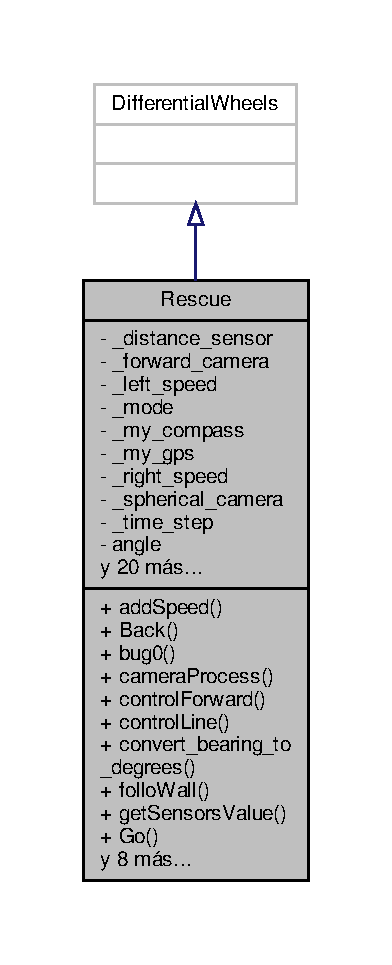
\includegraphics[width=188pt]{classRescue__inherit__graph}
\end{center}
\end{figure}


Diagrama de colaboración para Rescue\+:\nopagebreak
\begin{figure}[H]
\begin{center}
\leavevmode
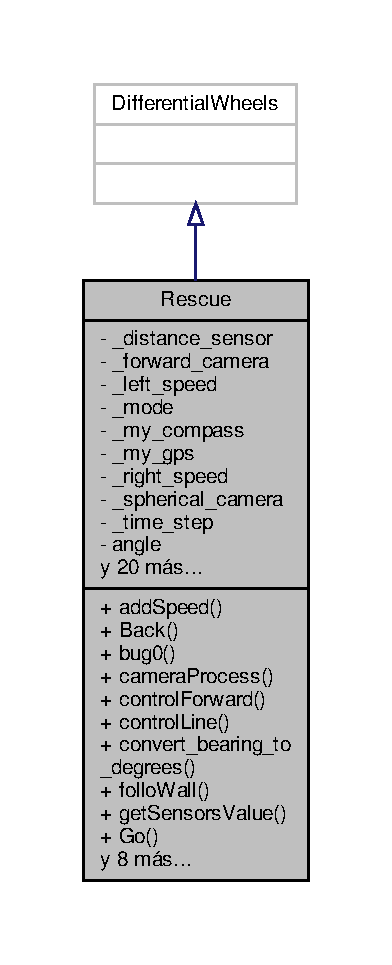
\includegraphics[width=188pt]{classRescue__coll__graph}
\end{center}
\end{figure}
\subsection*{Métodos públicos}
\begin{DoxyCompactItemize}
\item 
void \hyperlink{classRescue_a9a430924f65d71eca4e02dc9b2704947_a9a430924f65d71eca4e02dc9b2704947}{add\+Speed} (double left\+\_\+speed, double right\+\_\+speed)
\begin{DoxyCompactList}\small\item\em Funcion para asignar un valor en concreto a los atributos \+\_\+left\+\_\+speed y \+\_\+right\+\_\+speed. \end{DoxyCompactList}\item 
void \hyperlink{classRescue_a5acc91c16b60baf09a87f440a22f030f_a5acc91c16b60baf09a87f440a22f030f}{Back} ()
\begin{DoxyCompactList}\small\item\em Tercer y último método principal de \hyperlink{classRescue}{Rescue}, llama a initial\+Position para situarse a 180º con respecto al mapa y según de donde haya venido, utilizará \hyperlink{classRescue_aa9f20abea5898b53b03db91f2a323982_aa9f20abea5898b53b03db91f2a323982}{follo\+Wall()} o \hyperlink{classRescue_a85cbbec8d486f16e260d3f74c3221831_a85cbbec8d486f16e260d3f74c3221831}{home\+Coming()}. \end{DoxyCompactList}\item 
void \hyperlink{classRescue_a4e3ec37a662b2cb91df3dcb0a875acf9_a4e3ec37a662b2cb91df3dcb0a875acf9}{bug0} ()
\begin{DoxyCompactList}\small\item\em Aplica la tecnica del bug0 en base a una posición objetivo y asigna un valor a deg que se actualiza cada vez que se llama. \end{DoxyCompactList}\item 
bool \hyperlink{classRescue_a8fca4fbd58ec9ccab6fc88424b16723f_a8fca4fbd58ec9ccab6fc88424b16723f}{camera\+Process} ()
\begin{DoxyCompactList}\small\item\em Método utilizado en \hyperlink{classRescue_a3ea9a01b97d0291afa704bff73564938_a3ea9a01b97d0291afa704bff73564938}{Search()}, este método, a igual que \hyperlink{classRescue_ab1ea1e98e62403dc681f26529805fe2a_ab1ea1e98e62403dc681f26529805fe2a}{yellow\+Line()},alaniza pixel por pixel para encontrar posibles objetivos de distinta tonalidad de verde y si encuentra, se moverá en dirección a donde se encuentra mediante la posición en de la imagen de la cámara en la que se encuentra.\+Devuelve un booleano si encuentra objetivos. \end{DoxyCompactList}\item 
void \hyperlink{classRescue_a47bd9c67c0e779f2dbf9ce6e5f81b831_a47bd9c67c0e779f2dbf9ce6e5f81b831}{control\+Forward} ()
\begin{DoxyCompactList}\small\item\em Funcion generalmente usada en modo F\+O\+R\+W\+A\+RD para manener una dirección concreta dada por el atributo angle.\+Si el robot se sale de ur rango en torno al valor de angle, este se corrige girando en sentido contrario hacia donde se mueve el robot por error En este ejemplo, seguirá una dirección en torno a 90º \+: \end{DoxyCompactList}\item 
void \hyperlink{classRescue_aeef91de334e7779ce2fb2c2b57cd70c3_aeef91de334e7779ce2fb2c2b57cd70c3}{control\+Line} ()
\begin{DoxyCompactList}\small\item\em Función principal para los modos del robot, cada vez que se llama, mira cual fue el ultimo modo activado y asigna unas ciertas velocidades a \hyperlink{classRescue_a9a430924f65d71eca4e02dc9b2704947_a9a430924f65d71eca4e02dc9b2704947}{add\+Speed()} segun el modo requerido.\+SI el modo es F\+O\+R\+W\+A\+RD, en la función llamará a control forward. \end{DoxyCompactList}\item 
double \hyperlink{classRescue_ac0d22bd4b26374b9eba3a229397b08a2_ac0d22bd4b26374b9eba3a229397b08a2}{convert\+\_\+bearing\+\_\+to\+\_\+degrees} (const double $\ast$in\+\_\+vector)
\begin{DoxyCompactList}\small\item\em Convierte los valores dados por el metodo get\+Values() de Compass en grados. \end{DoxyCompactList}\item 
void \hyperlink{classRescue_aa9f20abea5898b53b03db91f2a323982_aa9f20abea5898b53b03db91f2a323982}{follo\+Wall} ()
\begin{DoxyCompactList}\small\item\em En este método, el robot sigue el muro con los sensores de distancia laterales esquivando obstáculos con los sesonres de distancia frontales. \end{DoxyCompactList}\item 
void \hyperlink{classRescue_a68675aa6bb37102baf46803451e16c82_a68675aa6bb37102baf46803451e16c82}{get\+Sensors\+Value} ()
\begin{DoxyCompactList}\small\item\em Cada vez que se llama, dará los valores de los sensores inicializados por el robot (exceptuando las cámaras) para su posterior tratamiento. \end{DoxyCompactList}\item 
void \hyperlink{classRescue_acfe79ba42004fd73e17e240c0201462a_acfe79ba42004fd73e17e240c0201462a}{Go} ()
\begin{DoxyCompactList}\small\item\em Primera función principal de las fases de Go,Search,Back. \end{DoxyCompactList}\item 
void \hyperlink{classRescue_a85cbbec8d486f16e260d3f74c3221831_a85cbbec8d486f16e260d3f74c3221831}{home\+Coming} ()
\begin{DoxyCompactList}\small\item\em Este método emplea la misma metodología que \hyperlink{classRescue_acfe79ba42004fd73e17e240c0201462a_acfe79ba42004fd73e17e240c0201462a}{Go()}, primero el robot debe ir al centro del mapa esquivando obstáculos con los sensores de distancia, el robot gira a la izquierda si se encuentra un obstaculo frontal. \end{DoxyCompactList}\item 
void \hyperlink{classRescue_a3c978120304fcdbe702f3e306bef6c02_a3c978120304fcdbe702f3e306bef6c02}{initial\+Position} (int angulo\+\_\+salida)
\begin{DoxyCompactList}\small\item\em Inicializa el robot a una orientación general dada por parametro a la ida(\+Go()) o vuelta (\hyperlink{classRescue_a5acc91c16b60baf09a87f440a22f030f_a5acc91c16b60baf09a87f440a22f030f}{Back()}) del mapa, permitiendo evitar errores de orientación. \end{DoxyCompactList}\item 
void \hyperlink{classRescue_a7db0c26d41013e7405311d2725efce86_a7db0c26d41013e7405311d2725efce86}{mapa\+Siete} ()
\begin{DoxyCompactList}\small\item\em Función especifia usada en \hyperlink{classRescue_acfe79ba42004fd73e17e240c0201462a_acfe79ba42004fd73e17e240c0201462a}{Go()}, indica una situación especial dada en el mapa de prueba scenario7 el cual en \hyperlink{classRescue_acfe79ba42004fd73e17e240c0201462a_acfe79ba42004fd73e17e240c0201462a}{Go()} el robot detectará si se encuentra en dicho mapa y llamará a esta función para desplazar el robot por dicho mapa mediante bug0. \end{DoxyCompactList}\item 
\hyperlink{classRescue_a307e122659d2fbe9e17f51108951752f_a307e122659d2fbe9e17f51108951752f}{Rescue} ()
\begin{DoxyCompactList}\small\item\em Contructor de la clase \hyperlink{classRescue}{Rescue}, inicializa todas las variables y habilita todos los sensores. \end{DoxyCompactList}\item 
vector$<$ float $>$ \hyperlink{classRescue_af2ba5b73069e7407f1bfc857a1ddae9c_af2ba5b73069e7407f1bfc857a1ddae9c}{R\+G\+B2\+H\+SV} (unsigned char \hyperlink{classRescue_af9ba54390762489e7f5c13ea8623b745_af9ba54390762489e7f5c13ea8623b745}{red}, unsigned char \hyperlink{classRescue_a5ec72c1115b4a89bd6079f74866b4717_a5ec72c1115b4a89bd6079f74866b4717}{green}, unsigned char \hyperlink{classRescue_adeb74390f710b4a180605f4a68e1bc77_adeb74390f710b4a180605f4a68e1bc77}{blue})
\begin{DoxyCompactList}\small\item\em Convierte el espacio de colores R\+GB a H\+SV para un reconocimiento mejor de colores. \end{DoxyCompactList}\item 
void \hyperlink{classRescue_a3ea9a01b97d0291afa704bff73564938_a3ea9a01b97d0291afa704bff73564938}{Search} ()
\begin{DoxyCompactList}\small\item\em Segundo método principar de la clase \hyperlink{classRescue}{Rescue}, en este método tiene como finalidad buscar dos objetivos o cilindros verdes por un area la cual no puede salir hasta haber encontrado a los objetivos. \end{DoxyCompactList}\item 
bool \hyperlink{classRescue_ab1ea1e98e62403dc681f26529805fe2a_ab1ea1e98e62403dc681f26529805fe2a}{yellow\+Line} ()
\begin{DoxyCompactList}\small\item\em Esta función es usada principalmente en Go, su función principal es la busqueda de la linea amarilla que indica que es la salida del mapa. \end{DoxyCompactList}\item 
\hyperlink{classRescue_a0330877161b533b15ea96b0daf85b692_a0330877161b533b15ea96b0daf85b692}{$\sim$\+Rescue} ()
\begin{DoxyCompactList}\small\item\em Usado para liberar la memoria de los sensores y resetear el robot a sus valores por defecto. \end{DoxyCompactList}\end{DoxyCompactItemize}
\subsection*{Tipos privados}
\begin{DoxyCompactItemize}
\item 
enum \hyperlink{classRescue_ab44ced9ce57b1b0d19b5456cd952d702_ab44ced9ce57b1b0d19b5456cd952d702}{Mode} \{ \newline
\hyperlink{classRescue_ab44ced9ce57b1b0d19b5456cd952d702_ab44ced9ce57b1b0d19b5456cd952d702a49eaffbbe22c056613ab9e4e52f63ad1}{S\+T\+OP}, 
\hyperlink{classRescue_ab44ced9ce57b1b0d19b5456cd952d702_ab44ced9ce57b1b0d19b5456cd952d702ac5b8fd2a28d3d22c89095ccb90ea6e2a}{F\+O\+R\+W\+A\+RD}, 
\hyperlink{classRescue_ab44ced9ce57b1b0d19b5456cd952d702_ab44ced9ce57b1b0d19b5456cd952d702ac001dd90d48926e098b61d39461bbe4d}{T\+U\+R\+N\+\_\+\+L\+E\+FT}, 
\hyperlink{classRescue_ab44ced9ce57b1b0d19b5456cd952d702_ab44ced9ce57b1b0d19b5456cd952d702aabd16068766c629e1f83fd217668a2e8}{T\+U\+R\+N\+\_\+\+R\+I\+G\+HT}, 
\newline
\hyperlink{classRescue_ab44ced9ce57b1b0d19b5456cd952d702_ab44ced9ce57b1b0d19b5456cd952d702afe3eef9ce0c9dc77b03e2cbeea734899}{T\+U\+R\+N\+\_\+\+L\+E\+F\+T\+\_\+\+C\+O\+N\+T\+R\+OL}, 
\hyperlink{classRescue_ab44ced9ce57b1b0d19b5456cd952d702_ab44ced9ce57b1b0d19b5456cd952d702ae5a7150c4e173fcb6aaf1d2082bf0081}{T\+U\+R\+N\+\_\+\+R\+I\+G\+H\+T\+\_\+\+C\+O\+N\+T\+R\+OL}
 \}\begin{DoxyCompactList}\small\item\em Modos de funcionamiento del robot\+: -\/\+S\+T\+OP\+:para el robot. \end{DoxyCompactList}
\end{DoxyCompactItemize}
\subsection*{Atributos privados}
\begin{DoxyCompactItemize}
\item 
Distance\+Sensor $\ast$ \hyperlink{classRescue_a1e1f6c1dc43593a25989127b6ca89ae9_a1e1f6c1dc43593a25989127b6ca89ae9}{\+\_\+distance\+\_\+sensor} \mbox{[}\hyperlink{Rescue_8h_a3bfa6c68d124846bd629eef1504b2556_a3bfa6c68d124846bd629eef1504b2556}{N\+U\+M\+\_\+\+D\+I\+S\+T\+A\+N\+C\+E\+\_\+\+S\+E\+N\+S\+OR}\mbox{]}
\item 
Camera $\ast$ \hyperlink{classRescue_a8cc51f98f8203494918ca1d313fca408_a8cc51f98f8203494918ca1d313fca408}{\+\_\+forward\+\_\+camera}
\item 
double \hyperlink{classRescue_a29d594459f17968e6db993605d239c47_a29d594459f17968e6db993605d239c47}{\+\_\+left\+\_\+speed}
\begin{DoxyCompactList}\small\item\em Velocidades de la rueda izquierda y derecha. \end{DoxyCompactList}\item 
\hyperlink{classRescue_ab44ced9ce57b1b0d19b5456cd952d702_ab44ced9ce57b1b0d19b5456cd952d702}{Mode} \hyperlink{classRescue_a70a5e292c84029568ff6c0de2f2d9f43_a70a5e292c84029568ff6c0de2f2d9f43}{\+\_\+mode}
\item 
Compass $\ast$ \hyperlink{classRescue_ab6c7e1a7c7cb23027b1d53aea73697b7_ab6c7e1a7c7cb23027b1d53aea73697b7}{\+\_\+my\+\_\+compass}
\item 
G\+PS $\ast$ \hyperlink{classRescue_ab3b6799de1bf84d1bf4a85afef8db0b2_ab3b6799de1bf84d1bf4a85afef8db0b2}{\+\_\+my\+\_\+gps}
\item 
double \hyperlink{classRescue_ab2fac6f0352d593bfc083709ecc9ddc1_ab2fac6f0352d593bfc083709ecc9ddc1}{\+\_\+right\+\_\+speed}
\item 
Camera $\ast$ \hyperlink{classRescue_a6f2788baf7717274fc75241b989796bc_a6f2788baf7717274fc75241b989796bc}{\+\_\+spherical\+\_\+camera}
\item 
int \hyperlink{classRescue_abbc48e2cca3b2acf36b530e5070f1756_abbc48e2cca3b2acf36b530e5070f1756}{\+\_\+time\+\_\+step}
\begin{DoxyCompactList}\small\item\em Tiempo de salto de la simulación. \end{DoxyCompactList}\item 
double \hyperlink{classRescue_a5bb8010f938dbe020a183b486772afe4_a5bb8010f938dbe020a183b486772afe4}{angle}
\begin{DoxyCompactList}\small\item\em Atributos de orientación del robot. \end{DoxyCompactList}\item 
double \hyperlink{classRescue_acc6616f1ab243e26c8903faca1cc7feb_acc6616f1ab243e26c8903faca1cc7feb}{B\+A\+C\+K\+\_\+X}
\begin{DoxyCompactList}\small\item\em Posiciónes x e y de llegada al final del mapa, indican por donde ha entado el robot. \end{DoxyCompactList}\item 
double \hyperlink{classRescue_aab2477ae06d7c87401e2306f36261120_aab2477ae06d7c87401e2306f36261120}{B\+A\+C\+K\+\_\+Y}
\item 
unsigned char \hyperlink{classRescue_adeb74390f710b4a180605f4a68e1bc77_adeb74390f710b4a180605f4a68e1bc77}{blue}
\item 
int \hyperlink{classRescue_a180e2955648c5bae24069da9db0c1a5f_a180e2955648c5bae24069da9db0c1a5f}{color\+\_\+counter}
\begin{DoxyCompactList}\small\item\em Contador de color para saltar de \hyperlink{classRescue_acfe79ba42004fd73e17e240c0201462a_acfe79ba42004fd73e17e240c0201462a}{Go()} a \hyperlink{classRescue_a3ea9a01b97d0291afa704bff73564938_a3ea9a01b97d0291afa704bff73564938}{Search()} \end{DoxyCompactList}\item 
double \hyperlink{classRescue_a5783a7f93b5dc970e997a919af57e0bc_a5783a7f93b5dc970e997a919af57e0bc}{compass}
\item 
double \hyperlink{classRescue_ad6febda0e181e1b6847e1b9be0f54e2b_ad6febda0e181e1b6847e1b9be0f54e2b}{deg}
\begin{DoxyCompactList}\small\item\em Angulo de bug0 del robot con respecto a la posición objetivo. \end{DoxyCompactList}\item 
int \hyperlink{classRescue_ab1e1f44c42138628cf62b8d56430e776_ab1e1f44c42138628cf62b8d56430e776}{dist\+\_\+sensor}
\begin{DoxyCompactList}\small\item\em Numeros de sensores activos. \end{DoxyCompactList}\item 
unsigned char \hyperlink{classRescue_a5ec72c1115b4a89bd6079f74866b4717_a5ec72c1115b4a89bd6079f74866b4717}{green}
\item 
double \hyperlink{classRescue_aaafc15a9b059bf1acbfa360915308fe5_aaafc15a9b059bf1acbfa360915308fe5}{ir\+\_\+val} \mbox{[}\hyperlink{Rescue_8h_a3bfa6c68d124846bd629eef1504b2556_a3bfa6c68d124846bd629eef1504b2556}{N\+U\+M\+\_\+\+D\+I\+S\+T\+A\+N\+C\+E\+\_\+\+S\+E\+N\+S\+OR}\mbox{]}
\begin{DoxyCompactList}\small\item\em Array de valores de los sensores de distancia. \end{DoxyCompactList}\item 
double \hyperlink{classRescue_aa1e9ec232ed1643bf2c889be84c8f4af_aa1e9ec232ed1643bf2c889be84c8f4af}{max} =0
\item 
double \hyperlink{classRescue_a8a98fdaa1deed080b4f8798f769f46cc_a8a98fdaa1deed080b4f8798f769f46cc}{O\+B\+J\+E\+C\+T\+I\+V\+E\+\_\+X}
\begin{DoxyCompactList}\small\item\em Objetivos correspondientes en cada punto del proceso, cambia según las fases o parte de ellas. \end{DoxyCompactList}\item 
double \hyperlink{classRescue_a54840a89d4f27081c433d70e1a78022f_a54840a89d4f27081c433d70e1a78022f}{O\+B\+J\+E\+C\+T\+I\+V\+E\+\_\+Y}
\item 
double \hyperlink{classRescue_a37191f058e32b0d1e8c184cfbf6daf5f_a37191f058e32b0d1e8c184cfbf6daf5f}{percentage\+\_\+green}
\begin{DoxyCompactList}\small\item\em Porcentaje de verde en la imagen de la camara frontal. \end{DoxyCompactList}\item 
double \hyperlink{classRescue_ad0101336342f1b5e9753b692d0d8b484_ad0101336342f1b5e9753b692d0d8b484}{percentage\+\_\+yellow}
\begin{DoxyCompactList}\small\item\em Porcentage de amarillo en la imagen. \end{DoxyCompactList}\item 
unsigned char \hyperlink{classRescue_af9ba54390762489e7f5c13ea8623b745_af9ba54390762489e7f5c13ea8623b745}{red}
\item 
int \hyperlink{classRescue_a92ae48ef6c0bb371cb0ea9c6eb4a8a87_a92ae48ef6c0bb371cb0ea9c6eb4a8a87}{sum\+\_\+l}
\begin{DoxyCompactList}\small\item\em Indicadores de dirección de la camara, indica por donde el robot debe ir en base a que mitad de la cámara se encuentra el objetivo. \end{DoxyCompactList}\item 
int \hyperlink{classRescue_af84f4ef8ca1595be05ebcd5907f06c25_af84f4ef8ca1595be05ebcd5907f06c25}{sum\+\_\+r}
\item 
int \hyperlink{classRescue_a9a95f0cd95b72a89f87c6e9b19d71f73_a9a95f0cd95b72a89f87c6e9b19d71f73}{sum\+\_\+y}
\begin{DoxyCompactList}\small\item\em Contador de pixeles amarillos en la imagen. \end{DoxyCompactList}\item 
double \hyperlink{classRescue_ab2a4cd163b6619df49346383bb08d365_ab2a4cd163b6619df49346383bb08d365}{X}
\begin{DoxyCompactList}\small\item\em Posicion de x con respecto al mapa. \end{DoxyCompactList}\item 
double \hyperlink{classRescue_aefe62362f68d14dc3f9234791de23882_aefe62362f68d14dc3f9234791de23882}{Y}
\begin{DoxyCompactList}\small\item\em Posición de y con respecto al mapa. \end{DoxyCompactList}\end{DoxyCompactItemize}


\subsection{Descripción detallada}
Controlador de un robot de busqueda y localización de dos personas en distintos tipos de escenarios. 

\begin{DoxyAuthor}{Autor}
Javier Galán Méndez 
\end{DoxyAuthor}
\begin{DoxyDate}{Fecha}
26-\/11-\/2019 
\end{DoxyDate}
\begin{DoxyVersion}{Versión}
1.\+0 
\end{DoxyVersion}


Definición en la línea 29 del archivo Rescue.\+h.



\subsection{Documentación de las enumeraciones miembro de la clase}
\mbox{\Hypertarget{classRescue_ab44ced9ce57b1b0d19b5456cd952d702_ab44ced9ce57b1b0d19b5456cd952d702}\label{classRescue_ab44ced9ce57b1b0d19b5456cd952d702_ab44ced9ce57b1b0d19b5456cd952d702}} 
\index{Rescue@{Rescue}!Mode@{Mode}}
\index{Mode@{Mode}!Rescue@{Rescue}}
\subsubsection{\texorpdfstring{Mode}{Mode}}
{\footnotesize\ttfamily enum \hyperlink{classRescue_ab44ced9ce57b1b0d19b5456cd952d702_ab44ced9ce57b1b0d19b5456cd952d702}{Rescue\+::\+Mode}\hspace{0.3cm}{\ttfamily [private]}}



Modos de funcionamiento del robot\+: -\/\+S\+T\+OP\+:para el robot. 

-\/\+F\+O\+R\+W\+A\+RD\+:el robot avanza hacia una dirección. -\/\+T\+U\+R\+N\+\_\+\+L\+E\+FT\+:gira en su eje vertical hacia la izquierda. -\/\+T\+U\+R\+N\+\_\+\+R\+I\+G\+HT\+:gira en su eje vertical hacia la derecha. -\/\+T\+U\+R\+N\+\_\+\+L\+E\+F\+T\+\_\+\+C\+O\+N\+T\+R\+OL\+:gira ligeramente hacia la izquierda-\/ -\/\+T\+U\+R\+N\+\_\+\+R\+I\+G\+H\+T\+\_\+\+C\+O\+N\+T\+R\+OL\+:gira ligeramente hacia la derecha. \begin{DoxyEnumFields}{Valores de enumeraciones}
\raisebox{\heightof{T}}[0pt][0pt]{\index{S\+T\+OP@{S\+T\+OP}!Rescue@{Rescue}}\index{Rescue@{Rescue}!S\+T\+OP@{S\+T\+OP}}}\mbox{\Hypertarget{classRescue_ab44ced9ce57b1b0d19b5456cd952d702_ab44ced9ce57b1b0d19b5456cd952d702a49eaffbbe22c056613ab9e4e52f63ad1}\label{classRescue_ab44ced9ce57b1b0d19b5456cd952d702_ab44ced9ce57b1b0d19b5456cd952d702a49eaffbbe22c056613ab9e4e52f63ad1}} 
S\+T\+OP&\\
\hline

\raisebox{\heightof{T}}[0pt][0pt]{\index{F\+O\+R\+W\+A\+RD@{F\+O\+R\+W\+A\+RD}!Rescue@{Rescue}}\index{Rescue@{Rescue}!F\+O\+R\+W\+A\+RD@{F\+O\+R\+W\+A\+RD}}}\mbox{\Hypertarget{classRescue_ab44ced9ce57b1b0d19b5456cd952d702_ab44ced9ce57b1b0d19b5456cd952d702ac5b8fd2a28d3d22c89095ccb90ea6e2a}\label{classRescue_ab44ced9ce57b1b0d19b5456cd952d702_ab44ced9ce57b1b0d19b5456cd952d702ac5b8fd2a28d3d22c89095ccb90ea6e2a}} 
F\+O\+R\+W\+A\+RD&\\
\hline

\raisebox{\heightof{T}}[0pt][0pt]{\index{T\+U\+R\+N\+\_\+\+L\+E\+FT@{T\+U\+R\+N\+\_\+\+L\+E\+FT}!Rescue@{Rescue}}\index{Rescue@{Rescue}!T\+U\+R\+N\+\_\+\+L\+E\+FT@{T\+U\+R\+N\+\_\+\+L\+E\+FT}}}\mbox{\Hypertarget{classRescue_ab44ced9ce57b1b0d19b5456cd952d702_ab44ced9ce57b1b0d19b5456cd952d702ac001dd90d48926e098b61d39461bbe4d}\label{classRescue_ab44ced9ce57b1b0d19b5456cd952d702_ab44ced9ce57b1b0d19b5456cd952d702ac001dd90d48926e098b61d39461bbe4d}} 
T\+U\+R\+N\+\_\+\+L\+E\+FT&\\
\hline

\raisebox{\heightof{T}}[0pt][0pt]{\index{T\+U\+R\+N\+\_\+\+R\+I\+G\+HT@{T\+U\+R\+N\+\_\+\+R\+I\+G\+HT}!Rescue@{Rescue}}\index{Rescue@{Rescue}!T\+U\+R\+N\+\_\+\+R\+I\+G\+HT@{T\+U\+R\+N\+\_\+\+R\+I\+G\+HT}}}\mbox{\Hypertarget{classRescue_ab44ced9ce57b1b0d19b5456cd952d702_ab44ced9ce57b1b0d19b5456cd952d702aabd16068766c629e1f83fd217668a2e8}\label{classRescue_ab44ced9ce57b1b0d19b5456cd952d702_ab44ced9ce57b1b0d19b5456cd952d702aabd16068766c629e1f83fd217668a2e8}} 
T\+U\+R\+N\+\_\+\+R\+I\+G\+HT&\\
\hline

\raisebox{\heightof{T}}[0pt][0pt]{\index{T\+U\+R\+N\+\_\+\+L\+E\+F\+T\+\_\+\+C\+O\+N\+T\+R\+OL@{T\+U\+R\+N\+\_\+\+L\+E\+F\+T\+\_\+\+C\+O\+N\+T\+R\+OL}!Rescue@{Rescue}}\index{Rescue@{Rescue}!T\+U\+R\+N\+\_\+\+L\+E\+F\+T\+\_\+\+C\+O\+N\+T\+R\+OL@{T\+U\+R\+N\+\_\+\+L\+E\+F\+T\+\_\+\+C\+O\+N\+T\+R\+OL}}}\mbox{\Hypertarget{classRescue_ab44ced9ce57b1b0d19b5456cd952d702_ab44ced9ce57b1b0d19b5456cd952d702afe3eef9ce0c9dc77b03e2cbeea734899}\label{classRescue_ab44ced9ce57b1b0d19b5456cd952d702_ab44ced9ce57b1b0d19b5456cd952d702afe3eef9ce0c9dc77b03e2cbeea734899}} 
T\+U\+R\+N\+\_\+\+L\+E\+F\+T\+\_\+\+C\+O\+N\+T\+R\+OL&\\
\hline

\raisebox{\heightof{T}}[0pt][0pt]{\index{T\+U\+R\+N\+\_\+\+R\+I\+G\+H\+T\+\_\+\+C\+O\+N\+T\+R\+OL@{T\+U\+R\+N\+\_\+\+R\+I\+G\+H\+T\+\_\+\+C\+O\+N\+T\+R\+OL}!Rescue@{Rescue}}\index{Rescue@{Rescue}!T\+U\+R\+N\+\_\+\+R\+I\+G\+H\+T\+\_\+\+C\+O\+N\+T\+R\+OL@{T\+U\+R\+N\+\_\+\+R\+I\+G\+H\+T\+\_\+\+C\+O\+N\+T\+R\+OL}}}\mbox{\Hypertarget{classRescue_ab44ced9ce57b1b0d19b5456cd952d702_ab44ced9ce57b1b0d19b5456cd952d702ae5a7150c4e173fcb6aaf1d2082bf0081}\label{classRescue_ab44ced9ce57b1b0d19b5456cd952d702_ab44ced9ce57b1b0d19b5456cd952d702ae5a7150c4e173fcb6aaf1d2082bf0081}} 
T\+U\+R\+N\+\_\+\+R\+I\+G\+H\+T\+\_\+\+C\+O\+N\+T\+R\+OL&\\
\hline

\end{DoxyEnumFields}


Definición en la línea 228 del archivo Rescue.\+h.


\begin{DoxyCode}
228                 \{
229             \hyperlink{classRescue_ab44ced9ce57b1b0d19b5456cd952d702_ab44ced9ce57b1b0d19b5456cd952d702a49eaffbbe22c056613ab9e4e52f63ad1}{STOP},
230             \hyperlink{classRescue_ab44ced9ce57b1b0d19b5456cd952d702_ab44ced9ce57b1b0d19b5456cd952d702ac5b8fd2a28d3d22c89095ccb90ea6e2a}{FORWARD},
231             \hyperlink{classRescue_ab44ced9ce57b1b0d19b5456cd952d702_ab44ced9ce57b1b0d19b5456cd952d702ac001dd90d48926e098b61d39461bbe4d}{TURN\_LEFT},
232             \hyperlink{classRescue_ab44ced9ce57b1b0d19b5456cd952d702_ab44ced9ce57b1b0d19b5456cd952d702aabd16068766c629e1f83fd217668a2e8}{TURN\_RIGHT},
233             \hyperlink{classRescue_ab44ced9ce57b1b0d19b5456cd952d702_ab44ced9ce57b1b0d19b5456cd952d702afe3eef9ce0c9dc77b03e2cbeea734899}{TURN\_LEFT\_CONTROL},
234             \hyperlink{classRescue_ab44ced9ce57b1b0d19b5456cd952d702_ab44ced9ce57b1b0d19b5456cd952d702ae5a7150c4e173fcb6aaf1d2082bf0081}{TURN\_RIGHT\_CONTROL}
235         \};
\end{DoxyCode}


\subsection{Documentación del constructor y destructor}
\mbox{\Hypertarget{classRescue_a307e122659d2fbe9e17f51108951752f_a307e122659d2fbe9e17f51108951752f}\label{classRescue_a307e122659d2fbe9e17f51108951752f_a307e122659d2fbe9e17f51108951752f}} 
\index{Rescue@{Rescue}!Rescue@{Rescue}}
\index{Rescue@{Rescue}!Rescue@{Rescue}}
\subsubsection{\texorpdfstring{Rescue()}{Rescue()}}
{\footnotesize\ttfamily Rescue\+::\+Rescue (\begin{DoxyParamCaption}{ }\end{DoxyParamCaption})}



Contructor de la clase \hyperlink{classRescue}{Rescue}, inicializa todas las variables y habilita todos los sensores. 

La velocidad del robot se inicializa en modo F\+O\+R\+W\+A\+RD, que andará recto. Es usado para crear un robot de busqueda 
\begin{DoxyCode}
\textcolor{keywordtype}{int} \hyperlink{Pioneer_8cpp_a3c04138a5bfe5d72780bb7e82a18e627_a3c04138a5bfe5d72780bb7e82a18e627}{main}()\{
  \hyperlink{classRescue}{Rescue} *mirobot=\textcolor{keyword}{new} \hyperlink{classRescue_a307e122659d2fbe9e17f51108951752f_a307e122659d2fbe9e17f51108951752f}{Rescue}();
\}
\end{DoxyCode}
 

Definición en la línea 10 del archivo Rescue.\+cpp.


\begin{DoxyCode}
10                : DifferentialWheels()
11 \{
12     \textcolor{comment}{// Inicializas valores de los atributos}
13     \hyperlink{classRescue_abbc48e2cca3b2acf36b530e5070f1756_abbc48e2cca3b2acf36b530e5070f1756}{\_time\_step} = 32;
14 
15     \hyperlink{classRescue_a29d594459f17968e6db993605d239c47_a29d594459f17968e6db993605d239c47}{\_left\_speed} = \hyperlink{Rescue_8h_ac2cd96d53dd3ba6407db6766c3d92b26_ac2cd96d53dd3ba6407db6766c3d92b26}{MAX\_SPEED};
16     \hyperlink{classRescue_ab2fac6f0352d593bfc083709ecc9ddc1_ab2fac6f0352d593bfc083709ecc9ddc1}{\_right\_speed} = \hyperlink{Rescue_8h_ac2cd96d53dd3ba6407db6766c3d92b26_ac2cd96d53dd3ba6407db6766c3d92b26}{MAX\_SPEED};
17   
18     \hyperlink{classRescue_a70a5e292c84029568ff6c0de2f2d9f43_a70a5e292c84029568ff6c0de2f2d9f43}{\_mode} = \hyperlink{classRescue_ab44ced9ce57b1b0d19b5456cd952d702_ab44ced9ce57b1b0d19b5456cd952d702ac5b8fd2a28d3d22c89095ccb90ea6e2a}{FORWARD};
19     \hyperlink{classRescue_a9a95f0cd95b72a89f87c6e9b19d71f73_a9a95f0cd95b72a89f87c6e9b19d71f73}{sum\_y}=0;
20     \hyperlink{classRescue_a5ec72c1115b4a89bd6079f74866b4717_a5ec72c1115b4a89bd6079f74866b4717}{green} = 0;
21     \hyperlink{classRescue_af9ba54390762489e7f5c13ea8623b745_af9ba54390762489e7f5c13ea8623b745}{red} = 0;
22     \hyperlink{classRescue_adeb74390f710b4a180605f4a68e1bc77_adeb74390f710b4a180605f4a68e1bc77}{blue} = 0;
23     \hyperlink{classRescue_a180e2955648c5bae24069da9db0c1a5f_a180e2955648c5bae24069da9db0c1a5f}{color\_counter}=0;
24     \hyperlink{classRescue_ad0101336342f1b5e9753b692d0d8b484_ad0101336342f1b5e9753b692d0d8b484}{percentage\_yellow}=0.0;
25     \hyperlink{classRescue_a37191f058e32b0d1e8c184cfbf6daf5f_a37191f058e32b0d1e8c184cfbf6daf5f}{percentage\_green}=0.0;
26     \hyperlink{classRescue_a8a98fdaa1deed080b4f8798f769f46cc_a8a98fdaa1deed080b4f8798f769f46cc}{OBJECTIVE\_X}=0.0;
27     \hyperlink{classRescue_a54840a89d4f27081c433d70e1a78022f_a54840a89d4f27081c433d70e1a78022f}{OBJECTIVE\_Y}=0.2;
28     \hyperlink{classRescue_acc6616f1ab243e26c8903faca1cc7feb_acc6616f1ab243e26c8903faca1cc7feb}{BACK\_X}=\hyperlink{classRescue_aab2477ae06d7c87401e2306f36261120_aab2477ae06d7c87401e2306f36261120}{BACK\_Y}=0;
29     \hyperlink{classRescue_a5bb8010f938dbe020a183b486772afe4_a5bb8010f938dbe020a183b486772afe4}{angle}=0;
30     \hyperlink{classRescue_a5783a7f93b5dc970e997a919af57e0bc_a5783a7f93b5dc970e997a919af57e0bc}{compass}=0;
31     \hyperlink{classRescue_a92ae48ef6c0bb371cb0ea9c6eb4a8a87_a92ae48ef6c0bb371cb0ea9c6eb4a8a87}{sum\_l}=0;
32     \hyperlink{classRescue_af84f4ef8ca1595be05ebcd5907f06c25_af84f4ef8ca1595be05ebcd5907f06c25}{sum\_r}=0;
33     \hyperlink{classRescue_ab2a4cd163b6619df49346383bb08d365_ab2a4cd163b6619df49346383bb08d365}{X} = \hyperlink{classRescue_aefe62362f68d14dc3f9234791de23882_aefe62362f68d14dc3f9234791de23882}{Y} = 0.0;
34     \hyperlink{classRescue_ad6febda0e181e1b6847e1b9be0f54e2b_ad6febda0e181e1b6847e1b9be0f54e2b}{deg}=0.0;
35     \textcolor{comment}{// Guradas los sensores en un array}
36     \textcolor{keywordflow}{for}(\textcolor{keywordtype}{int} i=0;i<\hyperlink{Rescue_8h_a3bfa6c68d124846bd629eef1504b2556_a3bfa6c68d124846bd629eef1504b2556}{NUM\_DISTANCE\_SENSOR};i++)\{
37       \textcolor{keywordtype}{string} str = to\_string(i);
38       \hyperlink{classRescue_a1e1f6c1dc43593a25989127b6ca89ae9_a1e1f6c1dc43593a25989127b6ca89ae9}{\_distance\_sensor}[i] = getDistanceSensor(\textcolor{stringliteral}{"ds"}+str);
39       \hyperlink{classRescue_a1e1f6c1dc43593a25989127b6ca89ae9_a1e1f6c1dc43593a25989127b6ca89ae9}{\_distance\_sensor}[i]->enable(\hyperlink{classRescue_abbc48e2cca3b2acf36b530e5070f1756_abbc48e2cca3b2acf36b530e5070f1756}{\_time\_step});
40     \}
41     \textcolor{comment}{//Obtienes los dispositivos y los habilitas}
42     \hyperlink{classRescue_ab6c7e1a7c7cb23027b1d53aea73697b7_ab6c7e1a7c7cb23027b1d53aea73697b7}{\_my\_compass}=getCompass(\textcolor{stringliteral}{"compass"});
43     \hyperlink{classRescue_ab6c7e1a7c7cb23027b1d53aea73697b7_ab6c7e1a7c7cb23027b1d53aea73697b7}{\_my\_compass}->enable(\hyperlink{classRescue_abbc48e2cca3b2acf36b530e5070f1756_abbc48e2cca3b2acf36b530e5070f1756}{\_time\_step});
44     \hyperlink{classRescue_ab3b6799de1bf84d1bf4a85afef8db0b2_ab3b6799de1bf84d1bf4a85afef8db0b2}{\_my\_gps}=getGPS(\textcolor{stringliteral}{"gps"});
45     \hyperlink{classRescue_ab3b6799de1bf84d1bf4a85afef8db0b2_ab3b6799de1bf84d1bf4a85afef8db0b2}{\_my\_gps}->enable(\hyperlink{classRescue_abbc48e2cca3b2acf36b530e5070f1756_abbc48e2cca3b2acf36b530e5070f1756}{\_time\_step});
46     \hyperlink{classRescue_a6f2788baf7717274fc75241b989796bc_a6f2788baf7717274fc75241b989796bc}{\_spherical\_camera} = getCamera(\textcolor{stringliteral}{"camera\_s"});
47     \hyperlink{classRescue_a6f2788baf7717274fc75241b989796bc_a6f2788baf7717274fc75241b989796bc}{\_spherical\_camera}->enable(\hyperlink{classRescue_abbc48e2cca3b2acf36b530e5070f1756_abbc48e2cca3b2acf36b530e5070f1756}{\_time\_step});
48     \hyperlink{classRescue_a8cc51f98f8203494918ca1d313fca408_a8cc51f98f8203494918ca1d313fca408}{\_forward\_camera} = getCamera(\textcolor{stringliteral}{"camera\_f"});
49     \hyperlink{classRescue_a8cc51f98f8203494918ca1d313fca408_a8cc51f98f8203494918ca1d313fca408}{\_forward\_camera}->enable(\hyperlink{classRescue_abbc48e2cca3b2acf36b530e5070f1756_abbc48e2cca3b2acf36b530e5070f1756}{\_time\_step});
50     
51     
52 \}
\end{DoxyCode}
\mbox{\Hypertarget{classRescue_a0330877161b533b15ea96b0daf85b692_a0330877161b533b15ea96b0daf85b692}\label{classRescue_a0330877161b533b15ea96b0daf85b692_a0330877161b533b15ea96b0daf85b692}} 
\index{Rescue@{Rescue}!````~Rescue@{$\sim$\+Rescue}}
\index{````~Rescue@{$\sim$\+Rescue}!Rescue@{Rescue}}
\subsubsection{\texorpdfstring{$\sim$\+Rescue()}{~Rescue()}}
{\footnotesize\ttfamily Rescue\+::$\sim$\+Rescue (\begin{DoxyParamCaption}{ }\end{DoxyParamCaption})}



Usado para liberar la memoria de los sensores y resetear el robot a sus valores por defecto. 

Se llama al usar la keyword delete a la clase creada 
\begin{DoxyCode}
\textcolor{keywordtype}{int} \hyperlink{Pioneer_8cpp_a3c04138a5bfe5d72780bb7e82a18e627_a3c04138a5bfe5d72780bb7e82a18e627}{main}()\{
  \hyperlink{classRescue}{Rescue} *mirobot=\textcolor{keyword}{new} \hyperlink{classRescue_a307e122659d2fbe9e17f51108951752f_a307e122659d2fbe9e17f51108951752f}{Rescue}();
  \textcolor{keyword}{delete} mirobot; 
\}
\end{DoxyCode}
 

Definición en la línea 56 del archivo Rescue.\+cpp.


\begin{DoxyCode}
57 \{
58     \textcolor{comment}{// Desactiva dispositivos y para el robot}
59     \hyperlink{classRescue_a6f2788baf7717274fc75241b989796bc_a6f2788baf7717274fc75241b989796bc}{\_spherical\_camera}->disable();
60     \textcolor{keywordflow}{for} (\textcolor{keywordtype}{int} i=0; i<\hyperlink{Rescue_8h_a3bfa6c68d124846bd629eef1504b2556_a3bfa6c68d124846bd629eef1504b2556}{NUM\_DISTANCE\_SENSOR}; i++) \{
61         \hyperlink{classRescue_a1e1f6c1dc43593a25989127b6ca89ae9_a1e1f6c1dc43593a25989127b6ca89ae9}{\_distance\_sensor}[i]->disable();
62     \}
63     \hyperlink{classRescue_ab6c7e1a7c7cb23027b1d53aea73697b7_ab6c7e1a7c7cb23027b1d53aea73697b7}{\_my\_compass}->disable();
64     \hyperlink{classRescue_ab3b6799de1bf84d1bf4a85afef8db0b2_ab3b6799de1bf84d1bf4a85afef8db0b2}{\_my\_gps}->disable();
65     this->disableEncoders();
66     \hyperlink{classRescue_a8cc51f98f8203494918ca1d313fca408_a8cc51f98f8203494918ca1d313fca408}{\_forward\_camera}->disable();
67     setSpeed(0.0,0.0);
68 \}
\end{DoxyCode}


\subsection{Documentación de las funciones miembro}
\mbox{\Hypertarget{classRescue_a9a430924f65d71eca4e02dc9b2704947_a9a430924f65d71eca4e02dc9b2704947}\label{classRescue_a9a430924f65d71eca4e02dc9b2704947_a9a430924f65d71eca4e02dc9b2704947}} 
\index{Rescue@{Rescue}!add\+Speed@{add\+Speed}}
\index{add\+Speed@{add\+Speed}!Rescue@{Rescue}}
\subsubsection{\texorpdfstring{add\+Speed()}{addSpeed()}}
{\footnotesize\ttfamily void Rescue\+::add\+Speed (\begin{DoxyParamCaption}\item[{double}]{left\+\_\+speed,  }\item[{double}]{right\+\_\+speed }\end{DoxyParamCaption})}



Funcion para asignar un valor en concreto a los atributos \+\_\+left\+\_\+speed y \+\_\+right\+\_\+speed. 


\begin{DoxyParams}{Parámetros}
{\em left\+\_\+speed} & Valor a asignar al atributo \+\_\+left\+\_\+speed \\
\hline
{\em right\+\_\+speed} & Valor a asignar al atributo \+\_\+right\+\_\+speed \\
\hline
\end{DoxyParams}


Definición en la línea 149 del archivo Rescue.\+cpp.


\begin{DoxyCode}
149                                                          \{
150       this->\hyperlink{classRescue_a29d594459f17968e6db993605d239c47_a29d594459f17968e6db993605d239c47}{\_left\_speed}=left\_speed;
151       this->\hyperlink{classRescue_ab2fac6f0352d593bfc083709ecc9ddc1_ab2fac6f0352d593bfc083709ecc9ddc1}{\_right\_speed}=right\_speed;
152 \}
\end{DoxyCode}
\mbox{\Hypertarget{classRescue_a5acc91c16b60baf09a87f440a22f030f_a5acc91c16b60baf09a87f440a22f030f}\label{classRescue_a5acc91c16b60baf09a87f440a22f030f_a5acc91c16b60baf09a87f440a22f030f}} 
\index{Rescue@{Rescue}!Back@{Back}}
\index{Back@{Back}!Rescue@{Rescue}}
\subsubsection{\texorpdfstring{Back()}{Back()}}
{\footnotesize\ttfamily void Rescue\+::\+Back (\begin{DoxyParamCaption}{ }\end{DoxyParamCaption})}



Tercer y último método principal de \hyperlink{classRescue}{Rescue}, llama a initial\+Position para situarse a 180º con respecto al mapa y según de donde haya venido, utilizará \hyperlink{classRescue_aa9f20abea5898b53b03db91f2a323982_aa9f20abea5898b53b03db91f2a323982}{follo\+Wall()} o \hyperlink{classRescue_a85cbbec8d486f16e260d3f74c3221831_a85cbbec8d486f16e260d3f74c3221831}{home\+Coming()}. 

El destino de las dos funciones es llegar al inicio del mapa y finalizar la seguencia cuando llege a dicho inicio. 

Definición en la línea 451 del archivo Rescue.\+cpp.


\begin{DoxyCode}
451                  \{
452    \hyperlink{classRescue_a180e2955648c5bae24069da9db0c1a5f_a180e2955648c5bae24069da9db0c1a5f}{color\_counter}=0;
453    \textcolor{keywordtype}{int} initial\_time=0;
454    \textcolor{keywordflow}{while}(step(\hyperlink{classRescue_abbc48e2cca3b2acf36b530e5070f1756_abbc48e2cca3b2acf36b530e5070f1756}{\_time\_step}) != -1 && \hyperlink{classRescue_ab2a4cd163b6619df49346383bb08d365_ab2a4cd163b6619df49346383bb08d365}{X}>-8.4)\{
455        \hyperlink{classRescue_a68675aa6bb37102baf46803451e16c82_a68675aa6bb37102baf46803451e16c82}{getSensorsValue}();
456        
457        \textcolor{keywordflow}{if}(initial\_time<25)\{
458          \textcolor{keywordflow}{if}(\hyperlink{classRescue_a5783a7f93b5dc970e997a919af57e0bc_a5783a7f93b5dc970e997a919af57e0bc}{compass}<0)\hyperlink{classRescue_a5783a7f93b5dc970e997a919af57e0bc_a5783a7f93b5dc970e997a919af57e0bc}{compass}+=360;
459          \hyperlink{classRescue_a3c978120304fcdbe702f3e306bef6c02_a3c978120304fcdbe702f3e306bef6c02}{initialPosition}(180);
460          initial\_time++;
461        \}
462        \textcolor{keywordflow}{else}\{
463        \textcolor{comment}{//Parte de abajo del mapa o parte de arriba}
464            \textcolor{keywordflow}{if}(\hyperlink{classRescue_aab2477ae06d7c87401e2306f36261120_aab2477ae06d7c87401e2306f36261120}{BACK\_Y}<-2.5) \hyperlink{classRescue_aa9f20abea5898b53b03db91f2a323982_aa9f20abea5898b53b03db91f2a323982}{folloWall}();
465            \textcolor{keywordflow}{else} \hyperlink{classRescue_a85cbbec8d486f16e260d3f74c3221831_a85cbbec8d486f16e260d3f74c3221831}{homeComing}();
466            \textcolor{keywordflow}{if}(\hyperlink{classRescue_a5783a7f93b5dc970e997a919af57e0bc_a5783a7f93b5dc970e997a919af57e0bc}{compass}<0)\hyperlink{classRescue_a5783a7f93b5dc970e997a919af57e0bc_a5783a7f93b5dc970e997a919af57e0bc}{compass}+=360;
467            \hyperlink{classRescue_aeef91de334e7779ce2fb2c2b57cd70c3_aeef91de334e7779ce2fb2c2b57cd70c3}{controlLine}();
468        \}
469        
470        
471        setSpeed(\hyperlink{classRescue_a29d594459f17968e6db993605d239c47_a29d594459f17968e6db993605d239c47}{\_left\_speed},\hyperlink{classRescue_ab2fac6f0352d593bfc083709ecc9ddc1_ab2fac6f0352d593bfc083709ecc9ddc1}{\_right\_speed});
472    \}
473 \}
\end{DoxyCode}
\mbox{\Hypertarget{classRescue_a4e3ec37a662b2cb91df3dcb0a875acf9_a4e3ec37a662b2cb91df3dcb0a875acf9}\label{classRescue_a4e3ec37a662b2cb91df3dcb0a875acf9_a4e3ec37a662b2cb91df3dcb0a875acf9}} 
\index{Rescue@{Rescue}!bug0@{bug0}}
\index{bug0@{bug0}!Rescue@{Rescue}}
\subsubsection{\texorpdfstring{bug0()}{bug0()}}
{\footnotesize\ttfamily void Rescue\+::bug0 (\begin{DoxyParamCaption}{ }\end{DoxyParamCaption})}



Aplica la tecnica del bug0 en base a una posición objetivo y asigna un valor a deg que se actualiza cada vez que se llama. 

Se suele usar en conjunto con control\+Forward. 
\begin{DoxyCode}
\hyperlink{classRescue_a4e3ec37a662b2cb91df3dcb0a875acf9_a4e3ec37a662b2cb91df3dcb0a875acf9}{bug0}();\textcolor{comment}{//Da un valor a deg}
\hyperlink{classRescue_a5bb8010f938dbe020a183b486772afe4_a5bb8010f938dbe020a183b486772afe4}{angle}=\hyperlink{classRescue_ad6febda0e181e1b6847e1b9be0f54e2b_ad6febda0e181e1b6847e1b9be0f54e2b}{deg};
\hyperlink{classRescue_a47bd9c67c0e779f2dbf9ce6e5f81b831_a47bd9c67c0e779f2dbf9ce6e5f81b831}{controlForward}();
\end{DoxyCode}
 La tecnica de bug0 es simple de aplicar, se da un objetivo al robot y este irá a ese objetivo tomando como referencia la dirección hacia el mismo. Mientras va, se deberán usar los sensores para esquivar objetos y usar \hyperlink{classRescue_aeef91de334e7779ce2fb2c2b57cd70c3_aeef91de334e7779ce2fb2c2b57cd70c3}{control\+Line()} para evitarlos 

Definición en la línea 176 del archivo Rescue.\+cpp.


\begin{DoxyCode}
176                  \{
177     \textcolor{comment}{//Obtiene los valores de los sensores}
178     \hyperlink{classRescue_a68675aa6bb37102baf46803451e16c82_a68675aa6bb37102baf46803451e16c82}{getSensorsValue}();
179     \textcolor{keywordtype}{double} delta\_x=\hyperlink{classRescue_a8a98fdaa1deed080b4f8798f769f46cc_a8a98fdaa1deed080b4f8798f769f46cc}{OBJECTIVE\_X}-\hyperlink{classRescue_ab2a4cd163b6619df49346383bb08d365_ab2a4cd163b6619df49346383bb08d365}{X};
180     \textcolor{keywordtype}{double} delta\_y=\hyperlink{classRescue_aefe62362f68d14dc3f9234791de23882_aefe62362f68d14dc3f9234791de23882}{Y}-\hyperlink{classRescue_a54840a89d4f27081c433d70e1a78022f_a54840a89d4f27081c433d70e1a78022f}{OBJECTIVE\_Y};
181     \textcolor{keywordtype}{double} rad=atan2(delta\_y,delta\_x);
182     \textcolor{comment}{//Pasas a grados}
183     \hyperlink{classRescue_ad6febda0e181e1b6847e1b9be0f54e2b_ad6febda0e181e1b6847e1b9be0f54e2b}{deg} = rad * (180.0 / M\_PI);
184     
185 \}
\end{DoxyCode}
\mbox{\Hypertarget{classRescue_a8fca4fbd58ec9ccab6fc88424b16723f_a8fca4fbd58ec9ccab6fc88424b16723f}\label{classRescue_a8fca4fbd58ec9ccab6fc88424b16723f_a8fca4fbd58ec9ccab6fc88424b16723f}} 
\index{Rescue@{Rescue}!camera\+Process@{camera\+Process}}
\index{camera\+Process@{camera\+Process}!Rescue@{Rescue}}
\subsubsection{\texorpdfstring{camera\+Process()}{cameraProcess()}}
{\footnotesize\ttfamily bool Rescue\+::camera\+Process (\begin{DoxyParamCaption}{ }\end{DoxyParamCaption})}



Método utilizado en \hyperlink{classRescue_a3ea9a01b97d0291afa704bff73564938_a3ea9a01b97d0291afa704bff73564938}{Search()}, este método, a igual que \hyperlink{classRescue_ab1ea1e98e62403dc681f26529805fe2a_ab1ea1e98e62403dc681f26529805fe2a}{yellow\+Line()},alaniza pixel por pixel para encontrar posibles objetivos de distinta tonalidad de verde y si encuentra, se moverá en dirección a donde se encuentra mediante la posición en de la imagen de la cámara en la que se encuentra.\+Devuelve un booleano si encuentra objetivos. 


\begin{DoxyCode}
\textcolor{keywordtype}{bool} verde=\textcolor{keyword}{false};
\textcolor{keywordflow}{while}(1)\{
  verde=\hyperlink{classRescue_a8fca4fbd58ec9ccab6fc88424b16723f_a8fca4fbd58ec9ccab6fc88424b16723f}{cameraProcess}();
  setSpeed(\hyperlink{classRescue_a29d594459f17968e6db993605d239c47_a29d594459f17968e6db993605d239c47}{\_left\_speed},\_right\_sped);
  \textcolor{keywordflow}{if}(verde==\textcolor{keyword}{true}) cout<<\textcolor{stringliteral}{"He encontrado objetivo"}<<endl;
\}
\end{DoxyCode}
 Este método usa \hyperlink{classRescue_a9a430924f65d71eca4e02dc9b2704947_a9a430924f65d71eca4e02dc9b2704947}{add\+Speed()} para mover el robot hacia el objeto, por lo que en la llamada debe estar set\+Speed(). 

Definición en la línea 394 del archivo Rescue.\+cpp.


\begin{DoxyCode}
394                           \{
395     \textcolor{keywordtype}{int} image\_width\_f = \hyperlink{classRescue_a8cc51f98f8203494918ca1d313fca408_a8cc51f98f8203494918ca1d313fca408}{\_forward\_camera}->getWidth();
396     \textcolor{keywordtype}{int} image\_height\_f = \hyperlink{classRescue_a8cc51f98f8203494918ca1d313fca408_a8cc51f98f8203494918ca1d313fca408}{\_forward\_camera}->getHeight();
397     vector<float>HVS;
398     \hyperlink{classRescue_a92ae48ef6c0bb371cb0ea9c6eb4a8a87_a92ae48ef6c0bb371cb0ea9c6eb4a8a87}{sum\_l}=0;
399     \hyperlink{classRescue_af84f4ef8ca1595be05ebcd5907f06c25_af84f4ef8ca1595be05ebcd5907f06c25}{sum\_r}=0;
400     \textcolor{keyword}{const} \textcolor{keywordtype}{unsigned} \textcolor{keywordtype}{char} *image\_f = \hyperlink{classRescue_a8cc51f98f8203494918ca1d313fca408_a8cc51f98f8203494918ca1d313fca408}{\_forward\_camera}->getImage();
401     \textcolor{keywordflow}{for}(\textcolor{keywordtype}{int} i=0;i<image\_width\_f;i++)\{
402         \textcolor{keywordflow}{for}(\textcolor{keywordtype}{int} j=0;j<image\_height\_f;j++)\{
403             \hyperlink{classRescue_a5ec72c1115b4a89bd6079f74866b4717_a5ec72c1115b4a89bd6079f74866b4717}{green}=\hyperlink{classRescue_a8cc51f98f8203494918ca1d313fca408_a8cc51f98f8203494918ca1d313fca408}{\_forward\_camera}->imageGetGreen(image\_f,image\_width\_f,i,j);
404             \hyperlink{classRescue_af9ba54390762489e7f5c13ea8623b745_af9ba54390762489e7f5c13ea8623b745}{red}=\hyperlink{classRescue_a8cc51f98f8203494918ca1d313fca408_a8cc51f98f8203494918ca1d313fca408}{\_forward\_camera}->imageGetRed(image\_f,image\_width\_f,i,j);
405             \hyperlink{classRescue_adeb74390f710b4a180605f4a68e1bc77_adeb74390f710b4a180605f4a68e1bc77}{blue}=\hyperlink{classRescue_a8cc51f98f8203494918ca1d313fca408_a8cc51f98f8203494918ca1d313fca408}{\_forward\_camera}->imageGetBlue(image\_f,image\_width\_f,i,j);
406             HVS=\hyperlink{classRescue_af2ba5b73069e7407f1bfc857a1ddae9c_af2ba5b73069e7407f1bfc857a1ddae9c}{RGB2HSV}(\hyperlink{classRescue_af9ba54390762489e7f5c13ea8623b745_af9ba54390762489e7f5c13ea8623b745}{red},\hyperlink{classRescue_a5ec72c1115b4a89bd6079f74866b4717_a5ec72c1115b4a89bd6079f74866b4717}{green},\hyperlink{classRescue_adeb74390f710b4a180605f4a68e1bc77_adeb74390f710b4a180605f4a68e1bc77}{blue});
407             \textcolor{keywordtype}{bool} SPACEH=HVS[0]>111 && HVS[0]<120;
408             \textcolor{keywordtype}{bool} SPACES=HVS[2]>0.2 && HVS[2]<=1;
409             \textcolor{keywordtype}{bool} SPACEV=HVS[1]>20 && HVS[1]<155;
410             \textcolor{keywordtype}{bool} GREEN=SPACEH==\textcolor{keyword}{true} && SPACES==\textcolor{keyword}{true} && SPACEV==\textcolor{keyword}{true};
411             \textcolor{comment}{//Lado de la cámara donde se encuentra el objetivo}
412             \textcolor{keywordflow}{if}(GREEN && i<=image\_width\_f/2) \hyperlink{classRescue_a92ae48ef6c0bb371cb0ea9c6eb4a8a87_a92ae48ef6c0bb371cb0ea9c6eb4a8a87}{sum\_l}++;
413             \textcolor{keywordflow}{else} \textcolor{keywordflow}{if}(GREEN && i>image\_width\_f/2) \hyperlink{classRescue_af84f4ef8ca1595be05ebcd5907f06c25_af84f4ef8ca1595be05ebcd5907f06c25}{sum\_r}++;
414             
415         \}
416       \}
417         \textcolor{comment}{//Control del robot por cámara}
418         \textcolor{keywordflow}{if}(\hyperlink{classRescue_a92ae48ef6c0bb371cb0ea9c6eb4a8a87_a92ae48ef6c0bb371cb0ea9c6eb4a8a87}{sum\_l}!=0 || \hyperlink{classRescue_af84f4ef8ca1595be05ebcd5907f06c25_af84f4ef8ca1595be05ebcd5907f06c25}{sum\_r}!=0)\{
419             \textcolor{keywordflow}{if}(\hyperlink{classRescue_a92ae48ef6c0bb371cb0ea9c6eb4a8a87_a92ae48ef6c0bb371cb0ea9c6eb4a8a87}{sum\_l}>\hyperlink{classRescue_af84f4ef8ca1595be05ebcd5907f06c25_af84f4ef8ca1595be05ebcd5907f06c25}{sum\_r}) \hyperlink{classRescue_a9a430924f65d71eca4e02dc9b2704947_a9a430924f65d71eca4e02dc9b2704947}{addSpeed}(50,60);
420             \textcolor{keywordflow}{else} \textcolor{keywordflow}{if}(\hyperlink{classRescue_a92ae48ef6c0bb371cb0ea9c6eb4a8a87_a92ae48ef6c0bb371cb0ea9c6eb4a8a87}{sum\_l}<\hyperlink{classRescue_af84f4ef8ca1595be05ebcd5907f06c25_af84f4ef8ca1595be05ebcd5907f06c25}{sum\_r}) \hyperlink{classRescue_a9a430924f65d71eca4e02dc9b2704947_a9a430924f65d71eca4e02dc9b2704947}{addSpeed}(60,50);
421             \textcolor{keywordflow}{else} \hyperlink{classRescue_a9a430924f65d71eca4e02dc9b2704947_a9a430924f65d71eca4e02dc9b2704947}{addSpeed}(90,90);
422             
423             \textcolor{keywordflow}{return} \textcolor{keyword}{true};
424         \}
425     
426       \textcolor{keywordflow}{return} \textcolor{keyword}{false};
427 \}
\end{DoxyCode}
\mbox{\Hypertarget{classRescue_a47bd9c67c0e779f2dbf9ce6e5f81b831_a47bd9c67c0e779f2dbf9ce6e5f81b831}\label{classRescue_a47bd9c67c0e779f2dbf9ce6e5f81b831_a47bd9c67c0e779f2dbf9ce6e5f81b831}} 
\index{Rescue@{Rescue}!control\+Forward@{control\+Forward}}
\index{control\+Forward@{control\+Forward}!Rescue@{Rescue}}
\subsubsection{\texorpdfstring{control\+Forward()}{controlForward()}}
{\footnotesize\ttfamily void Rescue\+::control\+Forward (\begin{DoxyParamCaption}{ }\end{DoxyParamCaption})}



Funcion generalmente usada en modo F\+O\+R\+W\+A\+RD para manener una dirección concreta dada por el atributo angle.\+Si el robot se sale de ur rango en torno al valor de angle, este se corrige girando en sentido contrario hacia donde se mueve el robot por error En este ejemplo, seguirá una dirección en torno a 90º \+: 


\begin{DoxyCode}
\textcolor{keywordflow}{if}(ir\_recto==\textcolor{keyword}{true})\{
   \hyperlink{classRescue_a70a5e292c84029568ff6c0de2f2d9f43_a70a5e292c84029568ff6c0de2f2d9f43}{\_mode}=\hyperlink{classRescue_ab44ced9ce57b1b0d19b5456cd952d702_ab44ced9ce57b1b0d19b5456cd952d702ac5b8fd2a28d3d22c89095ccb90ea6e2a}{FORWARD};
   \hyperlink{classRescue_a5bb8010f938dbe020a183b486772afe4_a5bb8010f938dbe020a183b486772afe4}{angle}=90;
   mirobot->controlForward();
\}
\end{DoxyCode}
 

Definición en la línea 103 del archivo Rescue.\+cpp.


\begin{DoxyCode}
103                            \{\textcolor{comment}{//Control del robot e torno a angle}
104     
105     \textcolor{keywordflow}{if}(\hyperlink{classRescue_a5783a7f93b5dc970e997a919af57e0bc_a5783a7f93b5dc970e997a919af57e0bc}{compass}<\hyperlink{classRescue_a5bb8010f938dbe020a183b486772afe4_a5bb8010f938dbe020a183b486772afe4}{angle}-1) \hyperlink{classRescue_a9a430924f65d71eca4e02dc9b2704947_a9a430924f65d71eca4e02dc9b2704947}{addSpeed}(\hyperlink{Rescue_8h_ac2cd96d53dd3ba6407db6766c3d92b26_ac2cd96d53dd3ba6407db6766c3d92b26}{MAX\_SPEED},
      \hyperlink{Rescue_8h_ac2cd96d53dd3ba6407db6766c3d92b26_ac2cd96d53dd3ba6407db6766c3d92b26}{MAX\_SPEED}/2);
106     \textcolor{keywordflow}{else} \textcolor{keywordflow}{if}(\hyperlink{classRescue_a5783a7f93b5dc970e997a919af57e0bc_a5783a7f93b5dc970e997a919af57e0bc}{compass}>(\hyperlink{classRescue_a5bb8010f938dbe020a183b486772afe4_a5bb8010f938dbe020a183b486772afe4}{angle}+1)) \hyperlink{classRescue_a9a430924f65d71eca4e02dc9b2704947_a9a430924f65d71eca4e02dc9b2704947}{addSpeed}(\hyperlink{Rescue_8h_ac2cd96d53dd3ba6407db6766c3d92b26_ac2cd96d53dd3ba6407db6766c3d92b26}{MAX\_SPEED}/2,
      \hyperlink{Rescue_8h_ac2cd96d53dd3ba6407db6766c3d92b26_ac2cd96d53dd3ba6407db6766c3d92b26}{MAX\_SPEED});
107     \textcolor{keywordflow}{else} \hyperlink{classRescue_a9a430924f65d71eca4e02dc9b2704947_a9a430924f65d71eca4e02dc9b2704947}{addSpeed}(\hyperlink{Rescue_8h_ac2cd96d53dd3ba6407db6766c3d92b26_ac2cd96d53dd3ba6407db6766c3d92b26}{MAX\_SPEED},\hyperlink{Rescue_8h_ac2cd96d53dd3ba6407db6766c3d92b26_ac2cd96d53dd3ba6407db6766c3d92b26}{MAX\_SPEED});
108     
109 \}
\end{DoxyCode}
\mbox{\Hypertarget{classRescue_aeef91de334e7779ce2fb2c2b57cd70c3_aeef91de334e7779ce2fb2c2b57cd70c3}\label{classRescue_aeef91de334e7779ce2fb2c2b57cd70c3_aeef91de334e7779ce2fb2c2b57cd70c3}} 
\index{Rescue@{Rescue}!control\+Line@{control\+Line}}
\index{control\+Line@{control\+Line}!Rescue@{Rescue}}
\subsubsection{\texorpdfstring{control\+Line()}{controlLine()}}
{\footnotesize\ttfamily void Rescue\+::control\+Line (\begin{DoxyParamCaption}{ }\end{DoxyParamCaption})}



Función principal para los modos del robot, cada vez que se llama, mira cual fue el ultimo modo activado y asigna unas ciertas velocidades a \hyperlink{classRescue_a9a430924f65d71eca4e02dc9b2704947_a9a430924f65d71eca4e02dc9b2704947}{add\+Speed()} segun el modo requerido.\+SI el modo es F\+O\+R\+W\+A\+RD, en la función llamará a control forward. 

En el ejemplo, el modo será girar a la derecha, por lo que llamará a add\+Speed(M\+A\+X\+S\+P\+E\+ED,-\/\+M\+A\+X\+S\+P\+E\+E\+D/2) para girar a la derecha\+: 
\begin{DoxyCode}
\hyperlink{classRescue_a70a5e292c84029568ff6c0de2f2d9f43_a70a5e292c84029568ff6c0de2f2d9f43}{\_mode}=\hyperlink{classRescue_ab44ced9ce57b1b0d19b5456cd952d702_ab44ced9ce57b1b0d19b5456cd952d702aabd16068766c629e1f83fd217668a2e8}{TURN\_RIGHT};
\hyperlink{classRescue_aeef91de334e7779ce2fb2c2b57cd70c3_aeef91de334e7779ce2fb2c2b57cd70c3}{controlLine}();
\end{DoxyCode}
 

Definición en la línea 71 del archivo Rescue.\+cpp.


\begin{DoxyCode}
71                         \{
72   \textcolor{keywordflow}{switch} (\hyperlink{classRescue_a70a5e292c84029568ff6c0de2f2d9f43_a70a5e292c84029568ff6c0de2f2d9f43}{\_mode})\{
73             \textcolor{keywordflow}{case} \hyperlink{classRescue_ab44ced9ce57b1b0d19b5456cd952d702_ab44ced9ce57b1b0d19b5456cd952d702a49eaffbbe22c056613ab9e4e52f63ad1}{STOP}:
74                 cout<<\textcolor{stringliteral}{"STOP"}<<endl;
75                 \hyperlink{classRescue_a9a430924f65d71eca4e02dc9b2704947_a9a430924f65d71eca4e02dc9b2704947}{addSpeed}(0,0);
76                 \textcolor{keywordflow}{break};
77             \textcolor{keywordflow}{case} \hyperlink{classRescue_ab44ced9ce57b1b0d19b5456cd952d702_ab44ced9ce57b1b0d19b5456cd952d702ac5b8fd2a28d3d22c89095ccb90ea6e2a}{FORWARD}:
78                 cout<<\textcolor{stringliteral}{"FORWARD"}<<endl;
79                 \hyperlink{classRescue_a47bd9c67c0e779f2dbf9ce6e5f81b831_a47bd9c67c0e779f2dbf9ce6e5f81b831}{controlForward}();
80                 \textcolor{keywordflow}{break};
81             \textcolor{keywordflow}{case} \hyperlink{classRescue_ab44ced9ce57b1b0d19b5456cd952d702_ab44ced9ce57b1b0d19b5456cd952d702ac001dd90d48926e098b61d39461bbe4d}{TURN\_LEFT}:
82                 cout<<\textcolor{stringliteral}{"TURN\_LEFT"}<<endl;
83                 \hyperlink{classRescue_a9a430924f65d71eca4e02dc9b2704947_a9a430924f65d71eca4e02dc9b2704947}{addSpeed}(-\hyperlink{Rescue_8h_ac2cd96d53dd3ba6407db6766c3d92b26_ac2cd96d53dd3ba6407db6766c3d92b26}{MAX\_SPEED}/2,\hyperlink{Rescue_8h_ac2cd96d53dd3ba6407db6766c3d92b26_ac2cd96d53dd3ba6407db6766c3d92b26}{MAX\_SPEED}/2);
84                 \textcolor{keywordflow}{break};
85             \textcolor{keywordflow}{case} \hyperlink{classRescue_ab44ced9ce57b1b0d19b5456cd952d702_ab44ced9ce57b1b0d19b5456cd952d702aabd16068766c629e1f83fd217668a2e8}{TURN\_RIGHT}:
86                 cout<<\textcolor{stringliteral}{"TURN\_RIGHT"}<<endl;
87                 \hyperlink{classRescue_a9a430924f65d71eca4e02dc9b2704947_a9a430924f65d71eca4e02dc9b2704947}{addSpeed}(\hyperlink{Rescue_8h_ac2cd96d53dd3ba6407db6766c3d92b26_ac2cd96d53dd3ba6407db6766c3d92b26}{MAX\_SPEED}/2,-\hyperlink{Rescue_8h_ac2cd96d53dd3ba6407db6766c3d92b26_ac2cd96d53dd3ba6407db6766c3d92b26}{MAX\_SPEED}/2);
88                 \textcolor{keywordflow}{break};
89             \textcolor{keywordflow}{case} \hyperlink{classRescue_ab44ced9ce57b1b0d19b5456cd952d702_ab44ced9ce57b1b0d19b5456cd952d702afe3eef9ce0c9dc77b03e2cbeea734899}{TURN\_LEFT\_CONTROL}:
90                 cout<<\textcolor{stringliteral}{"TURN\_LEFT\_CONTROL"}<<endl;
91                 \hyperlink{classRescue_a9a430924f65d71eca4e02dc9b2704947_a9a430924f65d71eca4e02dc9b2704947}{addSpeed}(\hyperlink{Rescue_8h_ac2cd96d53dd3ba6407db6766c3d92b26_ac2cd96d53dd3ba6407db6766c3d92b26}{MAX\_SPEED}/2,\hyperlink{Rescue_8h_ac2cd96d53dd3ba6407db6766c3d92b26_ac2cd96d53dd3ba6407db6766c3d92b26}{MAX\_SPEED});
92                 \textcolor{keywordflow}{break};
93             \textcolor{keywordflow}{case} \hyperlink{classRescue_ab44ced9ce57b1b0d19b5456cd952d702_ab44ced9ce57b1b0d19b5456cd952d702ae5a7150c4e173fcb6aaf1d2082bf0081}{TURN\_RIGHT\_CONTROL}:
94                 cout<<\textcolor{stringliteral}{"TURN\_RIGHT\_CONTROL"}<<endl;
95                 \hyperlink{classRescue_a9a430924f65d71eca4e02dc9b2704947_a9a430924f65d71eca4e02dc9b2704947}{addSpeed}(\hyperlink{Rescue_8h_ac2cd96d53dd3ba6407db6766c3d92b26_ac2cd96d53dd3ba6407db6766c3d92b26}{MAX\_SPEED},\hyperlink{Rescue_8h_ac2cd96d53dd3ba6407db6766c3d92b26_ac2cd96d53dd3ba6407db6766c3d92b26}{MAX\_SPEED}/2);
96                 \textcolor{keywordflow}{break};
97             \textcolor{keywordflow}{default}:
98                 \textcolor{keywordflow}{break};
99         \}
100 \}
\end{DoxyCode}
\mbox{\Hypertarget{classRescue_ac0d22bd4b26374b9eba3a229397b08a2_ac0d22bd4b26374b9eba3a229397b08a2}\label{classRescue_ac0d22bd4b26374b9eba3a229397b08a2_ac0d22bd4b26374b9eba3a229397b08a2}} 
\index{Rescue@{Rescue}!convert\+\_\+bearing\+\_\+to\+\_\+degrees@{convert\+\_\+bearing\+\_\+to\+\_\+degrees}}
\index{convert\+\_\+bearing\+\_\+to\+\_\+degrees@{convert\+\_\+bearing\+\_\+to\+\_\+degrees}!Rescue@{Rescue}}
\subsubsection{\texorpdfstring{convert\+\_\+bearing\+\_\+to\+\_\+degrees()}{convert\_bearing\_to\_degrees()}}
{\footnotesize\ttfamily double Rescue\+::convert\+\_\+bearing\+\_\+to\+\_\+degrees (\begin{DoxyParamCaption}\item[{const double $\ast$}]{in\+\_\+vector }\end{DoxyParamCaption})}



Convierte los valores dados por el metodo get\+Values() de Compass en grados. 


\begin{DoxyParams}{Parámetros}
{\em in\+\_\+vector} & Vector de valores de compass que se tratan con funciones de math.\+h para pasarlos a radianes y a grados \\
\hline
\end{DoxyParams}


Definición en la línea 261 del archivo Rescue.\+cpp.


\begin{DoxyCode}
262 \{
263     \textcolor{keywordtype}{double} rad = atan2(in\_vector[0], in\_vector[2]);
264     \textcolor{keywordtype}{double} degr = rad * (180.0 / M\_PI);
265 
266     \textcolor{keywordflow}{return} degr;
267 \}
\end{DoxyCode}
\mbox{\Hypertarget{classRescue_aa9f20abea5898b53b03db91f2a323982_aa9f20abea5898b53b03db91f2a323982}\label{classRescue_aa9f20abea5898b53b03db91f2a323982_aa9f20abea5898b53b03db91f2a323982}} 
\index{Rescue@{Rescue}!follo\+Wall@{follo\+Wall}}
\index{follo\+Wall@{follo\+Wall}!Rescue@{Rescue}}
\subsubsection{\texorpdfstring{follo\+Wall()}{folloWall()}}
{\footnotesize\ttfamily void Rescue\+::follo\+Wall (\begin{DoxyParamCaption}{ }\end{DoxyParamCaption})}



En este método, el robot sigue el muro con los sensores de distancia laterales esquivando obstáculos con los sesonres de distancia frontales. 



Definición en la línea 475 del archivo Rescue.\+cpp.


\begin{DoxyCode}
475                       \{
476 \textcolor{comment}{//Control del seguimiento del muro}
477    \textcolor{keywordtype}{bool} MURO\_IZQUIERDA=\hyperlink{classRescue_aaafc15a9b059bf1acbfa360915308fe5_aaafc15a9b059bf1acbfa360915308fe5}{ir\_val}[3]>0 || \hyperlink{classRescue_aaafc15a9b059bf1acbfa360915308fe5_aaafc15a9b059bf1acbfa360915308fe5}{ir\_val}[4]>0;
478    \textcolor{keywordtype}{bool} MURO\_FRONTAL=\hyperlink{classRescue_aaafc15a9b059bf1acbfa360915308fe5_aaafc15a9b059bf1acbfa360915308fe5}{ir\_val}[0]>400 && \hyperlink{classRescue_aaafc15a9b059bf1acbfa360915308fe5_aaafc15a9b059bf1acbfa360915308fe5}{ir\_val}[15]>400;
479    \textcolor{keywordtype}{bool} ESQUINA=ir\_val[1]>0;
480    \textcolor{keywordflow}{if}(MURO\_FRONTAL)\hyperlink{classRescue_a70a5e292c84029568ff6c0de2f2d9f43_a70a5e292c84029568ff6c0de2f2d9f43}{\_mode}=\hyperlink{classRescue_ab44ced9ce57b1b0d19b5456cd952d702_ab44ced9ce57b1b0d19b5456cd952d702aabd16068766c629e1f83fd217668a2e8}{TURN\_RIGHT};
481    \textcolor{keywordflow}{else} \textcolor{keywordflow}{if}(MURO\_IZQUIERDA)\{
482        \textcolor{keywordflow}{if}(ir\_val[3]>ir\_val[4])\hyperlink{classRescue_a70a5e292c84029568ff6c0de2f2d9f43_a70a5e292c84029568ff6c0de2f2d9f43}{\_mode}=\hyperlink{classRescue_ab44ced9ce57b1b0d19b5456cd952d702_ab44ced9ce57b1b0d19b5456cd952d702ae5a7150c4e173fcb6aaf1d2082bf0081}{TURN\_RIGHT\_CONTROL};
483        \textcolor{keywordflow}{else} \textcolor{keywordflow}{if}(ir\_val[3]<ir\_val[4])\hyperlink{classRescue_a70a5e292c84029568ff6c0de2f2d9f43_a70a5e292c84029568ff6c0de2f2d9f43}{\_mode}=\hyperlink{classRescue_ab44ced9ce57b1b0d19b5456cd952d702_ab44ced9ce57b1b0d19b5456cd952d702afe3eef9ce0c9dc77b03e2cbeea734899}{TURN\_LEFT\_CONTROL};
484        \textcolor{keywordflow}{else} \hyperlink{classRescue_a70a5e292c84029568ff6c0de2f2d9f43_a70a5e292c84029568ff6c0de2f2d9f43}{\_mode}=\hyperlink{classRescue_ab44ced9ce57b1b0d19b5456cd952d702_ab44ced9ce57b1b0d19b5456cd952d702ac5b8fd2a28d3d22c89095ccb90ea6e2a}{FORWARD};
485    \}
486    \textcolor{keywordflow}{else} \textcolor{keywordflow}{if}(ESQUINA)\hyperlink{classRescue_a70a5e292c84029568ff6c0de2f2d9f43_a70a5e292c84029568ff6c0de2f2d9f43}{\_mode}=\hyperlink{classRescue_ab44ced9ce57b1b0d19b5456cd952d702_ab44ced9ce57b1b0d19b5456cd952d702ae5a7150c4e173fcb6aaf1d2082bf0081}{TURN\_RIGHT\_CONTROL};
487 \}
\end{DoxyCode}
\mbox{\Hypertarget{classRescue_a68675aa6bb37102baf46803451e16c82_a68675aa6bb37102baf46803451e16c82}\label{classRescue_a68675aa6bb37102baf46803451e16c82_a68675aa6bb37102baf46803451e16c82}} 
\index{Rescue@{Rescue}!get\+Sensors\+Value@{get\+Sensors\+Value}}
\index{get\+Sensors\+Value@{get\+Sensors\+Value}!Rescue@{Rescue}}
\subsubsection{\texorpdfstring{get\+Sensors\+Value()}{getSensorsValue()}}
{\footnotesize\ttfamily void Rescue\+::get\+Sensors\+Value (\begin{DoxyParamCaption}{ }\end{DoxyParamCaption})}



Cada vez que se llama, dará los valores de los sensores inicializados por el robot (exceptuando las cámaras) para su posterior tratamiento. 

Ejemplo\+: 
\begin{DoxyCode}
   mi\_robot-> \hyperlink{classRescue_a68675aa6bb37102baf46803451e16c82_a68675aa6bb37102baf46803451e16c82}{getSensorsValue}();
   cout<<\textcolor{stringliteral}{"Compass:"}<<\hyperlink{classRescue_a5783a7f93b5dc970e997a919af57e0bc_a5783a7f93b5dc970e997a919af57e0bc}{compass}<<endl;
   cout<<\textcolor{stringliteral}{"X:"}<<\hyperlink{classRescue_ab2a4cd163b6619df49346383bb08d365_ab2a4cd163b6619df49346383bb08d365}{X}<<\textcolor{stringliteral}{", Y:"}<<\hyperlink{classRescue_aefe62362f68d14dc3f9234791de23882_aefe62362f68d14dc3f9234791de23882}{Y}<<endl;
   cout<<\textcolor{stringliteral}{"Valor sensor de distancia 0:"}<<ir\_val[0]<<endl;
\}
\end{DoxyCode}
 

Definición en la línea 154 del archivo Rescue.\+cpp.


\begin{DoxyCode}
154                             \{
155   \textcolor{keyword}{const} \textcolor{keywordtype}{double} *gps\_value;
156   \textcolor{keyword}{const} \textcolor{keywordtype}{double} *compass\_value;
157   \textcolor{comment}{//Valores del gps}
158   gps\_value=\hyperlink{classRescue_ab3b6799de1bf84d1bf4a85afef8db0b2_ab3b6799de1bf84d1bf4a85afef8db0b2}{\_my\_gps}->getValues();
159   \hyperlink{classRescue_ab2a4cd163b6619df49346383bb08d365_ab2a4cd163b6619df49346383bb08d365}{X}=gps\_value[2];
160   \hyperlink{classRescue_aefe62362f68d14dc3f9234791de23882_aefe62362f68d14dc3f9234791de23882}{Y}=gps\_value[0];
161   \textcolor{comment}{//Valores de la brújula   }
162   compass\_value=\hyperlink{classRescue_ab6c7e1a7c7cb23027b1d53aea73697b7_ab6c7e1a7c7cb23027b1d53aea73697b7}{\_my\_compass}->getValues();
163   \hyperlink{classRescue_a5783a7f93b5dc970e997a919af57e0bc_a5783a7f93b5dc970e997a919af57e0bc}{compass} = \hyperlink{classRescue_ac0d22bd4b26374b9eba3a229397b08a2_ac0d22bd4b26374b9eba3a229397b08a2}{convert\_bearing\_to\_degrees}(compass\_value)-45;
164   \textcolor{comment}{//Valores de los sensores delanteros de distancia}
165   \hyperlink{classRescue_ab1e1f44c42138628cf62b8d56430e776_ab1e1f44c42138628cf62b8d56430e776}{dist\_sensor}=0;
166   \textcolor{keywordflow}{for}(\textcolor{keywordtype}{int} i=0;i<5;i++)\{
167      \hyperlink{classRescue_aaafc15a9b059bf1acbfa360915308fe5_aaafc15a9b059bf1acbfa360915308fe5}{ir\_val}[i] = \hyperlink{classRescue_a1e1f6c1dc43593a25989127b6ca89ae9_a1e1f6c1dc43593a25989127b6ca89ae9}{\_distance\_sensor}[i]->getValue();
168      \textcolor{keywordflow}{if}(\hyperlink{classRescue_aaafc15a9b059bf1acbfa360915308fe5_aaafc15a9b059bf1acbfa360915308fe5}{ir\_val}[i]>0) \hyperlink{classRescue_ab1e1f44c42138628cf62b8d56430e776_ab1e1f44c42138628cf62b8d56430e776}{dist\_sensor}++;
169   \}
170   \textcolor{keywordflow}{for}(\textcolor{keywordtype}{int} i=11;i<=15;i++)\{
171       \hyperlink{classRescue_aaafc15a9b059bf1acbfa360915308fe5_aaafc15a9b059bf1acbfa360915308fe5}{ir\_val}[i] = \hyperlink{classRescue_a1e1f6c1dc43593a25989127b6ca89ae9_a1e1f6c1dc43593a25989127b6ca89ae9}{\_distance\_sensor}[i]->getValue();
172       \textcolor{keywordflow}{if}(\hyperlink{classRescue_aaafc15a9b059bf1acbfa360915308fe5_aaafc15a9b059bf1acbfa360915308fe5}{ir\_val}[i]>0) \hyperlink{classRescue_ab1e1f44c42138628cf62b8d56430e776_ab1e1f44c42138628cf62b8d56430e776}{dist\_sensor}++;
173   \}
174 \}
\end{DoxyCode}
\mbox{\Hypertarget{classRescue_acfe79ba42004fd73e17e240c0201462a_acfe79ba42004fd73e17e240c0201462a}\label{classRescue_acfe79ba42004fd73e17e240c0201462a_acfe79ba42004fd73e17e240c0201462a}} 
\index{Rescue@{Rescue}!Go@{Go}}
\index{Go@{Go}!Rescue@{Rescue}}
\subsubsection{\texorpdfstring{Go()}{Go()}}
{\footnotesize\ttfamily void Rescue\+::\+Go (\begin{DoxyParamCaption}{ }\end{DoxyParamCaption})}



Primera función principal de las fases de Go,Search,Back. 

En esta fase, se ha aplicado un bug0 en torno al centro del mapa (0,0) e irá hacia ese objetivo esquivando obstaculos mediante las diferentes situaciones y valores de los sensores de distancia del robot. Al parar ese objetivo (X$>$0), el robot tendrá como dirección la de la salida del mapa, es decir, donde supuestamente se encuentran los objetivos. El robot puede tomar direrentes rutas según como se encuentren los obtáculos, las principales salidas que suele tomar son la central y la de abajo, el cual esta ultima tendrá que dar media vuelta para poder entrar por el pasillo que conduce hacia dicha salida. Go se suele utilizar principalmente en el main, y Go llamará a las correspondientes funciones para realizar su correcto funcionamiento. Go termina cuando \hyperlink{classRescue_ab1ea1e98e62403dc681f26529805fe2a_ab1ea1e98e62403dc681f26529805fe2a}{yellow\+Line()} devuelve un true, indicando que ha llegado a la salida. 

Definición en la línea 200 del archivo Rescue.\+cpp.


\begin{DoxyCode}
201 \{
202     \textcolor{keywordtype}{bool} mapa7=\textcolor{keyword}{false};\textcolor{comment}{//Indica si el robot se encuentra en scenario7}
203     \textcolor{keywordtype}{double} time=0;
204     \textcolor{keywordtype}{bool} line=\textcolor{keyword}{false};\textcolor{comment}{//Marca si ha detectado linea amarilla}
205     \textcolor{keywordflow}{while} (step(\hyperlink{classRescue_abbc48e2cca3b2acf36b530e5070f1756_abbc48e2cca3b2acf36b530e5070f1756}{\_time\_step}) != -1 && line==\textcolor{keyword}{false}) \{
206         cout<<\hyperlink{classRescue_a5bb8010f938dbe020a183b486772afe4_a5bb8010f938dbe020a183b486772afe4}{angle}<<endl;
207         \hyperlink{classRescue_a68675aa6bb37102baf46803451e16c82_a68675aa6bb37102baf46803451e16c82}{getSensorsValue}();
208         \textcolor{keywordflow}{if}(\hyperlink{classRescue_aefe62362f68d14dc3f9234791de23882_aefe62362f68d14dc3f9234791de23882}{Y}<-2.35287 && \hyperlink{classRescue_ab2a4cd163b6619df49346383bb08d365_ab2a4cd163b6619df49346383bb08d365}{X}<-6) mapa7=\textcolor{keyword}{true};
209         \textcolor{keywordflow}{if}((\textcolor{keywordtype}{int})\hyperlink{classRescue_a5783a7f93b5dc970e997a919af57e0bc_a5783a7f93b5dc970e997a919af57e0bc}{compass}%180==0) \hyperlink{classRescue_a5bb8010f938dbe020a183b486772afe4_a5bb8010f938dbe020a183b486772afe4}{angle}=(int)\hyperlink{classRescue_a5783a7f93b5dc970e997a919af57e0bc_a5783a7f93b5dc970e997a919af57e0bc}{compass};
210         \textcolor{keywordflow}{if}((\textcolor{keywordtype}{int})\hyperlink{classRescue_a5783a7f93b5dc970e997a919af57e0bc_a5783a7f93b5dc970e997a919af57e0bc}{compass}>=-180 && (int)\hyperlink{classRescue_a5783a7f93b5dc970e997a919af57e0bc_a5783a7f93b5dc970e997a919af57e0bc}{compass}<-160) \hyperlink{classRescue_a5bb8010f938dbe020a183b486772afe4_a5bb8010f938dbe020a183b486772afe4}{angle}=-180;
211         \textcolor{comment}{//Distintas situaciones en el recorrido}
212         \textcolor{keywordtype}{bool} OBSTACULO\_FRONTAL=\hyperlink{classRescue_aaafc15a9b059bf1acbfa360915308fe5_aaafc15a9b059bf1acbfa360915308fe5}{ir\_val}[0]>0 && \hyperlink{classRescue_aaafc15a9b059bf1acbfa360915308fe5_aaafc15a9b059bf1acbfa360915308fe5}{ir\_val}[15]>0 && (angle<10 && angle>-10);
213         \textcolor{keywordtype}{bool} RINCON\_IZQUIERDA=\hyperlink{classRescue_aaafc15a9b059bf1acbfa360915308fe5_aaafc15a9b059bf1acbfa360915308fe5}{ir\_val}[0]>0 && \hyperlink{classRescue_aaafc15a9b059bf1acbfa360915308fe5_aaafc15a9b059bf1acbfa360915308fe5}{ir\_val}[3]>0;
214         \textcolor{keywordtype}{bool} MURO\_IZQUIERDA=ir\_val[3]>800 ;
215         \textcolor{keywordtype}{bool} MURO\_DERECHA=ir\_val[12]>800;
216         \textcolor{keywordtype}{bool} GIRA\_NORTE\_180= \hyperlink{classRescue_ab1e1f44c42138628cf62b8d56430e776_ab1e1f44c42138628cf62b8d56430e776}{dist\_sensor}==0 && (\hyperlink{classRescue_a5783a7f93b5dc970e997a919af57e0bc_a5783a7f93b5dc970e997a919af57e0bc}{compass}>170 || 
      \hyperlink{classRescue_a5783a7f93b5dc970e997a919af57e0bc_a5783a7f93b5dc970e997a919af57e0bc}{compass}<-170);
217         \textcolor{keywordtype}{bool} ESQUINA\_DERECHA=(ir\_val[15]>0 || ir\_val[12]>500) ;
218         \textcolor{keywordtype}{bool} PRUEBA=ir\_val[14]>0;
219         \textcolor{keywordtype}{bool} ESQUINA\_IZQUIERDA=(ir\_val[0]>0 || ir\_val[1]>0) && OBSTACULO\_FRONTAL==\textcolor{keyword}{false} ;
220         \textcolor{comment}{//Distintos actos según la situación obtenida a lo largo del mapa}
221         \textcolor{keywordflow}{if}(OBSTACULO\_FRONTAL)\hyperlink{classRescue_a70a5e292c84029568ff6c0de2f2d9f43_a70a5e292c84029568ff6c0de2f2d9f43}{\_mode}=\hyperlink{classRescue_ab44ced9ce57b1b0d19b5456cd952d702_ab44ced9ce57b1b0d19b5456cd952d702aabd16068766c629e1f83fd217668a2e8}{TURN\_RIGHT};
222         \textcolor{keywordflow}{else} \textcolor{keywordflow}{if}(MURO\_IZQUIERDA)\{
223             \textcolor{keywordflow}{if}(ir\_val[3]>ir\_val[4]) \hyperlink{classRescue_a70a5e292c84029568ff6c0de2f2d9f43_a70a5e292c84029568ff6c0de2f2d9f43}{\_mode}=\hyperlink{classRescue_ab44ced9ce57b1b0d19b5456cd952d702_ab44ced9ce57b1b0d19b5456cd952d702ae5a7150c4e173fcb6aaf1d2082bf0081}{TURN\_RIGHT\_CONTROL};
224             \textcolor{keywordflow}{else} \textcolor{keywordflow}{if}(ir\_val[3]<ir\_val[4] ) \hyperlink{classRescue_a70a5e292c84029568ff6c0de2f2d9f43_a70a5e292c84029568ff6c0de2f2d9f43}{\_mode}=\hyperlink{classRescue_ab44ced9ce57b1b0d19b5456cd952d702_ab44ced9ce57b1b0d19b5456cd952d702afe3eef9ce0c9dc77b03e2cbeea734899}{TURN\_LEFT\_CONTROL};
225             \textcolor{keywordflow}{else} \hyperlink{classRescue_a70a5e292c84029568ff6c0de2f2d9f43_a70a5e292c84029568ff6c0de2f2d9f43}{\_mode}=\hyperlink{classRescue_ab44ced9ce57b1b0d19b5456cd952d702_ab44ced9ce57b1b0d19b5456cd952d702ac5b8fd2a28d3d22c89095ccb90ea6e2a}{FORWARD};
226         \}
227         \textcolor{keywordflow}{else} \textcolor{keywordflow}{if}(MURO\_DERECHA)\{
228             \textcolor{keywordflow}{if}(ir\_val[11]>=ir\_val[12]) \hyperlink{classRescue_a70a5e292c84029568ff6c0de2f2d9f43_a70a5e292c84029568ff6c0de2f2d9f43}{\_mode}=\hyperlink{classRescue_ab44ced9ce57b1b0d19b5456cd952d702_ab44ced9ce57b1b0d19b5456cd952d702ae5a7150c4e173fcb6aaf1d2082bf0081}{TURN\_RIGHT\_CONTROL};
229             \textcolor{keywordflow}{else} \hyperlink{classRescue_a70a5e292c84029568ff6c0de2f2d9f43_a70a5e292c84029568ff6c0de2f2d9f43}{\_mode}=\hyperlink{classRescue_ab44ced9ce57b1b0d19b5456cd952d702_ab44ced9ce57b1b0d19b5456cd952d702afe3eef9ce0c9dc77b03e2cbeea734899}{TURN\_LEFT\_CONTROL};
230         \}
231         \textcolor{keywordflow}{else} \textcolor{keywordflow}{if}(ESQUINA\_DERECHA || PRUEBA)\hyperlink{classRescue_a70a5e292c84029568ff6c0de2f2d9f43_a70a5e292c84029568ff6c0de2f2d9f43}{\_mode}=\hyperlink{classRescue_ab44ced9ce57b1b0d19b5456cd952d702_ab44ced9ce57b1b0d19b5456cd952d702afe3eef9ce0c9dc77b03e2cbeea734899}{TURN\_LEFT\_CONTROL};
232         \textcolor{keywordflow}{else} \textcolor{keywordflow}{if}(ESQUINA\_IZQUIERDA)\hyperlink{classRescue_a70a5e292c84029568ff6c0de2f2d9f43_a70a5e292c84029568ff6c0de2f2d9f43}{\_mode}=\hyperlink{classRescue_ab44ced9ce57b1b0d19b5456cd952d702_ab44ced9ce57b1b0d19b5456cd952d702ae5a7150c4e173fcb6aaf1d2082bf0081}{TURN\_RIGHT\_CONTROL};
233         \textcolor{keywordflow}{else} \hyperlink{classRescue_a70a5e292c84029568ff6c0de2f2d9f43_a70a5e292c84029568ff6c0de2f2d9f43}{\_mode}=\hyperlink{classRescue_ab44ced9ce57b1b0d19b5456cd952d702_ab44ced9ce57b1b0d19b5456cd952d702ac5b8fd2a28d3d22c89095ccb90ea6e2a}{FORWARD};
234         \textcolor{comment}{//Eventos con prioridad}
235         \textcolor{keywordflow}{if}(\hyperlink{classRescue_ab1e1f44c42138628cf62b8d56430e776_ab1e1f44c42138628cf62b8d56430e776}{dist\_sensor}==0 && \hyperlink{classRescue_ab2a4cd163b6619df49346383bb08d365_ab2a4cd163b6619df49346383bb08d365}{X}<=0)\{
236             \hyperlink{classRescue_a70a5e292c84029568ff6c0de2f2d9f43_a70a5e292c84029568ff6c0de2f2d9f43}{\_mode}=\hyperlink{classRescue_ab44ced9ce57b1b0d19b5456cd952d702_ab44ced9ce57b1b0d19b5456cd952d702ac5b8fd2a28d3d22c89095ccb90ea6e2a}{FORWARD};
237             \hyperlink{classRescue_a5bb8010f938dbe020a183b486772afe4_a5bb8010f938dbe020a183b486772afe4}{angle}=\hyperlink{classRescue_ad6febda0e181e1b6847e1b9be0f54e2b_ad6febda0e181e1b6847e1b9be0f54e2b}{deg};
238         \}
239         \textcolor{keywordflow}{if}( GIRA\_NORTE\_180) \hyperlink{classRescue_a70a5e292c84029568ff6c0de2f2d9f43_a70a5e292c84029568ff6c0de2f2d9f43}{\_mode}=\hyperlink{classRescue_ab44ced9ce57b1b0d19b5456cd952d702_ab44ced9ce57b1b0d19b5456cd952d702afe3eef9ce0c9dc77b03e2cbeea734899}{TURN\_LEFT\_CONTROL};
240         \textcolor{keywordflow}{if}(mapa7==\textcolor{keyword}{true})\hyperlink{classRescue_a7db0c26d41013e7405311d2725efce86_a7db0c26d41013e7405311d2725efce86}{mapaSiete}();
241         \hyperlink{classRescue_a4e3ec37a662b2cb91df3dcb0a875acf9_a4e3ec37a662b2cb91df3dcb0a875acf9}{bug0}();
242         \textcolor{comment}{//Evita que en ciertos lugares del mapa cometa errores como al inicio o en una parte del mapa 7}
243         \textcolor{keywordflow}{if}(\hyperlink{classRescue_ab2a4cd163b6619df49346383bb08d365_ab2a4cd163b6619df49346383bb08d365}{X}>-7)line=\hyperlink{classRescue_ab1ea1e98e62403dc681f26529805fe2a_ab1ea1e98e62403dc681f26529805fe2a}{yellowLine}();
244         \textcolor{keywordflow}{if}(\hyperlink{classRescue_ab2a4cd163b6619df49346383bb08d365_ab2a4cd163b6619df49346383bb08d365}{X}>7.5 && mapa7==\textcolor{keyword}{true}) line=\textcolor{keyword}{true};
245         \textcolor{comment}{//Llamada a función del robot}
246         \hyperlink{classRescue_aeef91de334e7779ce2fb2c2b57cd70c3_aeef91de334e7779ce2fb2c2b57cd70c3}{controlLine}();
247         \textcolor{comment}{//Prioridad no controlada con controlLine()}
248         \textcolor{keywordflow}{if}(RINCON\_IZQUIERDA)\hyperlink{classRescue_a9a430924f65d71eca4e02dc9b2704947_a9a430924f65d71eca4e02dc9b2704947}{addSpeed}(30,-30);
249         \textcolor{comment}{//Orientación inicial}
250         \textcolor{keywordflow}{if}(time<=45 && (compass<-2 || compass>2)) \hyperlink{classRescue_a3c978120304fcdbe702f3e306bef6c02_a3c978120304fcdbe702f3e306bef6c02}{initialPosition}(0);
251        
252         \textcolor{comment}{// Establece las velocidades de los motores del robot}
253         setSpeed(\hyperlink{classRescue_a29d594459f17968e6db993605d239c47_a29d594459f17968e6db993605d239c47}{\_left\_speed},\hyperlink{classRescue_ab2fac6f0352d593bfc083709ecc9ddc1_ab2fac6f0352d593bfc083709ecc9ddc1}{\_right\_speed});
254         time++;
255     \}
256     \textcolor{comment}{//Aññade las ubicaciones desde donde ha entrado el robot a la área de busqueda de las personas}
257     \hyperlink{classRescue_a8a98fdaa1deed080b4f8798f769f46cc_a8a98fdaa1deed080b4f8798f769f46cc}{OBJECTIVE\_X}=\hyperlink{classRescue_acc6616f1ab243e26c8903faca1cc7feb_acc6616f1ab243e26c8903faca1cc7feb}{BACK\_X}=\hyperlink{classRescue_ab2a4cd163b6619df49346383bb08d365_ab2a4cd163b6619df49346383bb08d365}{X};
258     \hyperlink{classRescue_a54840a89d4f27081c433d70e1a78022f_a54840a89d4f27081c433d70e1a78022f}{OBJECTIVE\_Y}=\hyperlink{classRescue_aab2477ae06d7c87401e2306f36261120_aab2477ae06d7c87401e2306f36261120}{BACK\_Y}=\hyperlink{classRescue_aefe62362f68d14dc3f9234791de23882_aefe62362f68d14dc3f9234791de23882}{Y};
259 \}
\end{DoxyCode}
\mbox{\Hypertarget{classRescue_a85cbbec8d486f16e260d3f74c3221831_a85cbbec8d486f16e260d3f74c3221831}\label{classRescue_a85cbbec8d486f16e260d3f74c3221831_a85cbbec8d486f16e260d3f74c3221831}} 
\index{Rescue@{Rescue}!home\+Coming@{home\+Coming}}
\index{home\+Coming@{home\+Coming}!Rescue@{Rescue}}
\subsubsection{\texorpdfstring{home\+Coming()}{homeComing()}}
{\footnotesize\ttfamily void Rescue\+::home\+Coming (\begin{DoxyParamCaption}{ }\end{DoxyParamCaption})}



Este método emplea la misma metodología que \hyperlink{classRescue_acfe79ba42004fd73e17e240c0201462a_acfe79ba42004fd73e17e240c0201462a}{Go()}, primero el robot debe ir al centro del mapa esquivando obstáculos con los sensores de distancia, el robot gira a la izquierda si se encuentra un obstaculo frontal. 

Despues de llegar al centro del mapa, el robot se le marca otro objetivo que será el inicio del mapa siguiendo la misma metodología. 

Definición en la línea 489 del archivo Rescue.\+cpp.


\begin{DoxyCode}
489                        \{
490   \textcolor{comment}{//Condiciones en el recorrido  }
491   \textcolor{keywordtype}{bool} OBSTACULO\_FRONTAL=\hyperlink{classRescue_aaafc15a9b059bf1acbfa360915308fe5_aaafc15a9b059bf1acbfa360915308fe5}{ir\_val}[0]>0 && \hyperlink{classRescue_aaafc15a9b059bf1acbfa360915308fe5_aaafc15a9b059bf1acbfa360915308fe5}{ir\_val}[15]>0 && \hyperlink{classRescue_ab2a4cd163b6619df49346383bb08d365_ab2a4cd163b6619df49346383bb08d365}{X}<=6;
492   \textcolor{keywordtype}{bool} MURO\_DERECHA= \hyperlink{classRescue_aaafc15a9b059bf1acbfa360915308fe5_aaafc15a9b059bf1acbfa360915308fe5}{ir\_val}[12]>800;
493   \textcolor{keywordtype}{bool} MURO\_IZQUIERDA=\hyperlink{classRescue_aaafc15a9b059bf1acbfa360915308fe5_aaafc15a9b059bf1acbfa360915308fe5}{ir\_val}[3]>800;
494   \textcolor{keywordtype}{bool} ESQUINA\_IZQUIERDA=\hyperlink{classRescue_aaafc15a9b059bf1acbfa360915308fe5_aaafc15a9b059bf1acbfa360915308fe5}{ir\_val}[1]>0;
495   \textcolor{keywordtype}{bool} ESQUINA\_DERECHA=\hyperlink{classRescue_aaafc15a9b059bf1acbfa360915308fe5_aaafc15a9b059bf1acbfa360915308fe5}{ir\_val}[14]>0;
496   \textcolor{comment}{//Manejo de las condiciones}
497   \textcolor{keywordflow}{if}(OBSTACULO\_FRONTAL) \hyperlink{classRescue_a70a5e292c84029568ff6c0de2f2d9f43_a70a5e292c84029568ff6c0de2f2d9f43}{\_mode}=\hyperlink{classRescue_ab44ced9ce57b1b0d19b5456cd952d702_ab44ced9ce57b1b0d19b5456cd952d702ac001dd90d48926e098b61d39461bbe4d}{TURN\_LEFT};
498   \textcolor{keywordflow}{else} \textcolor{keywordflow}{if}(ESQUINA\_DERECHA)\hyperlink{classRescue_a70a5e292c84029568ff6c0de2f2d9f43_a70a5e292c84029568ff6c0de2f2d9f43}{\_mode}=\hyperlink{classRescue_ab44ced9ce57b1b0d19b5456cd952d702_ab44ced9ce57b1b0d19b5456cd952d702afe3eef9ce0c9dc77b03e2cbeea734899}{TURN\_LEFT\_CONTROL};
499   \textcolor{keywordflow}{else} \textcolor{keywordflow}{if}(ESQUINA\_IZQUIERDA)\hyperlink{classRescue_a70a5e292c84029568ff6c0de2f2d9f43_a70a5e292c84029568ff6c0de2f2d9f43}{\_mode}=\hyperlink{classRescue_ab44ced9ce57b1b0d19b5456cd952d702_ab44ced9ce57b1b0d19b5456cd952d702ae5a7150c4e173fcb6aaf1d2082bf0081}{TURN\_RIGHT\_CONTROL};
500   \textcolor{keywordflow}{else} \textcolor{keywordflow}{if}(MURO\_DERECHA)\{
501   
502     \textcolor{keywordflow}{if}(\hyperlink{classRescue_aaafc15a9b059bf1acbfa360915308fe5_aaafc15a9b059bf1acbfa360915308fe5}{ir\_val}[12]>\hyperlink{classRescue_aaafc15a9b059bf1acbfa360915308fe5_aaafc15a9b059bf1acbfa360915308fe5}{ir\_val}[11])\hyperlink{classRescue_a70a5e292c84029568ff6c0de2f2d9f43_a70a5e292c84029568ff6c0de2f2d9f43}{\_mode}=\hyperlink{classRescue_ab44ced9ce57b1b0d19b5456cd952d702_ab44ced9ce57b1b0d19b5456cd952d702afe3eef9ce0c9dc77b03e2cbeea734899}{TURN\_LEFT\_CONTROL};
503     \textcolor{keywordflow}{else} \textcolor{keywordflow}{if}(\hyperlink{classRescue_aaafc15a9b059bf1acbfa360915308fe5_aaafc15a9b059bf1acbfa360915308fe5}{ir\_val}[12]<\hyperlink{classRescue_aaafc15a9b059bf1acbfa360915308fe5_aaafc15a9b059bf1acbfa360915308fe5}{ir\_val}[11])\hyperlink{classRescue_a70a5e292c84029568ff6c0de2f2d9f43_a70a5e292c84029568ff6c0de2f2d9f43}{\_mode}=\hyperlink{classRescue_ab44ced9ce57b1b0d19b5456cd952d702_ab44ced9ce57b1b0d19b5456cd952d702ae5a7150c4e173fcb6aaf1d2082bf0081}{TURN\_RIGHT\_CONTROL};
504     \textcolor{keywordflow}{else} \hyperlink{classRescue_a70a5e292c84029568ff6c0de2f2d9f43_a70a5e292c84029568ff6c0de2f2d9f43}{\_mode}=\hyperlink{classRescue_ab44ced9ce57b1b0d19b5456cd952d702_ab44ced9ce57b1b0d19b5456cd952d702ac5b8fd2a28d3d22c89095ccb90ea6e2a}{FORWARD};
505     
506   \}
507   \textcolor{keywordflow}{else} \textcolor{keywordflow}{if}(MURO\_IZQUIERDA)\{
508     \textcolor{keywordflow}{if}(\hyperlink{classRescue_aaafc15a9b059bf1acbfa360915308fe5_aaafc15a9b059bf1acbfa360915308fe5}{ir\_val}[4]>\hyperlink{classRescue_aaafc15a9b059bf1acbfa360915308fe5_aaafc15a9b059bf1acbfa360915308fe5}{ir\_val}[3])\hyperlink{classRescue_a70a5e292c84029568ff6c0de2f2d9f43_a70a5e292c84029568ff6c0de2f2d9f43}{\_mode}=\hyperlink{classRescue_ab44ced9ce57b1b0d19b5456cd952d702_ab44ced9ce57b1b0d19b5456cd952d702afe3eef9ce0c9dc77b03e2cbeea734899}{TURN\_LEFT\_CONTROL};
509     \textcolor{keywordflow}{else} \textcolor{keywordflow}{if}(\hyperlink{classRescue_aaafc15a9b059bf1acbfa360915308fe5_aaafc15a9b059bf1acbfa360915308fe5}{ir\_val}[4]<\hyperlink{classRescue_aaafc15a9b059bf1acbfa360915308fe5_aaafc15a9b059bf1acbfa360915308fe5}{ir\_val}[3])\hyperlink{classRescue_a70a5e292c84029568ff6c0de2f2d9f43_a70a5e292c84029568ff6c0de2f2d9f43}{\_mode}=\hyperlink{classRescue_ab44ced9ce57b1b0d19b5456cd952d702_ab44ced9ce57b1b0d19b5456cd952d702ae5a7150c4e173fcb6aaf1d2082bf0081}{TURN\_RIGHT\_CONTROL};
510     \textcolor{keywordflow}{else} \hyperlink{classRescue_a70a5e292c84029568ff6c0de2f2d9f43_a70a5e292c84029568ff6c0de2f2d9f43}{\_mode}=\hyperlink{classRescue_ab44ced9ce57b1b0d19b5456cd952d702_ab44ced9ce57b1b0d19b5456cd952d702ac5b8fd2a28d3d22c89095ccb90ea6e2a}{FORWARD};
511   \}
512   \textcolor{comment}{//Establecimiento de objetivos y bug0}
513   \textcolor{keywordflow}{if}(\hyperlink{classRescue_ab1e1f44c42138628cf62b8d56430e776_ab1e1f44c42138628cf62b8d56430e776}{dist\_sensor}==0)\{
514      \textcolor{keywordflow}{if}(X<1)\{
515       \hyperlink{classRescue_a8a98fdaa1deed080b4f8798f769f46cc_a8a98fdaa1deed080b4f8798f769f46cc}{OBJECTIVE\_X}=-8;
516       \hyperlink{classRescue_a54840a89d4f27081c433d70e1a78022f_a54840a89d4f27081c433d70e1a78022f}{OBJECTIVE\_Y}=-0.65;
517      \}
518      \textcolor{keywordflow}{else}\{
519        \hyperlink{classRescue_a8a98fdaa1deed080b4f8798f769f46cc_a8a98fdaa1deed080b4f8798f769f46cc}{OBJECTIVE\_X}=1;
520       \hyperlink{classRescue_a54840a89d4f27081c433d70e1a78022f_a54840a89d4f27081c433d70e1a78022f}{OBJECTIVE\_Y}=0;
521      \}
522      \hyperlink{classRescue_a4e3ec37a662b2cb91df3dcb0a875acf9_a4e3ec37a662b2cb91df3dcb0a875acf9}{bug0}();
523      \hyperlink{classRescue_a70a5e292c84029568ff6c0de2f2d9f43_a70a5e292c84029568ff6c0de2f2d9f43}{\_mode}=\hyperlink{classRescue_ab44ced9ce57b1b0d19b5456cd952d702_ab44ced9ce57b1b0d19b5456cd952d702ac5b8fd2a28d3d22c89095ccb90ea6e2a}{FORWARD};
524      \textcolor{keywordflow}{if}(\hyperlink{classRescue_ad6febda0e181e1b6847e1b9be0f54e2b_ad6febda0e181e1b6847e1b9be0f54e2b}{deg}<0)\hyperlink{classRescue_ad6febda0e181e1b6847e1b9be0f54e2b_ad6febda0e181e1b6847e1b9be0f54e2b}{deg}+=360;
525      \hyperlink{classRescue_a5bb8010f938dbe020a183b486772afe4_a5bb8010f938dbe020a183b486772afe4}{angle}=\hyperlink{classRescue_ad6febda0e181e1b6847e1b9be0f54e2b_ad6febda0e181e1b6847e1b9be0f54e2b}{deg};
526      
527   \}
528 \}
\end{DoxyCode}
\mbox{\Hypertarget{classRescue_a3c978120304fcdbe702f3e306bef6c02_a3c978120304fcdbe702f3e306bef6c02}\label{classRescue_a3c978120304fcdbe702f3e306bef6c02_a3c978120304fcdbe702f3e306bef6c02}} 
\index{Rescue@{Rescue}!initial\+Position@{initial\+Position}}
\index{initial\+Position@{initial\+Position}!Rescue@{Rescue}}
\subsubsection{\texorpdfstring{initial\+Position()}{initialPosition()}}
{\footnotesize\ttfamily void Rescue\+::initial\+Position (\begin{DoxyParamCaption}\item[{int}]{angulo\+\_\+salida }\end{DoxyParamCaption})}



Inicializa el robot a una orientación general dada por parametro a la ida(\+Go()) o vuelta (\hyperlink{classRescue_a5acc91c16b60baf09a87f440a22f030f_a5acc91c16b60baf09a87f440a22f030f}{Back()}) del mapa, permitiendo evitar errores de orientación. 

Orienta el robot dando unas velocidades a \hyperlink{classRescue_a9a430924f65d71eca4e02dc9b2704947_a9a430924f65d71eca4e02dc9b2704947}{add\+Speed()} 
\begin{DoxyCode}
\textcolor{keywordflow}{while}(1)\{
    \textcolor{keywordflow}{if}(time<45)\{\textcolor{comment}{//Al inicio, el robot girará hasta estar orientado a 0º}
        \hyperlink{classRescue_a3c978120304fcdbe702f3e306bef6c02_a3c978120304fcdbe702f3e306bef6c02}{initialPosition}(0);
        time++;
    \}
    setSpeed(\hyperlink{classRescue_a29d594459f17968e6db993605d239c47_a29d594459f17968e6db993605d239c47}{\_left\_speed},\hyperlink{classRescue_ab2fac6f0352d593bfc083709ecc9ddc1_ab2fac6f0352d593bfc083709ecc9ddc1}{\_right\_speed});\textcolor{comment}{//Método de DifferentialWheels para dar una
       velocidad al robot;}
\}
\end{DoxyCode}
 
\begin{DoxyParams}{Parámetros}
{\em angulo\+\_\+salida} & angulo dado en la llamada a la que se quiere iniciar el robot \\
\hline
\end{DoxyParams}


Definición en la línea 194 del archivo Rescue.\+cpp.


\begin{DoxyCode}
194                                              \{
195   
196     \textcolor{keywordflow}{if}(compass<angulo\_salida-2 && compass>=angulo\_salida-180) \hyperlink{classRescue_a9a430924f65d71eca4e02dc9b2704947_a9a430924f65d71eca4e02dc9b2704947}{addSpeed}(
      \hyperlink{Rescue_8h_ac2cd96d53dd3ba6407db6766c3d92b26_ac2cd96d53dd3ba6407db6766c3d92b26}{MAX\_SPEED}/2,-\hyperlink{Rescue_8h_ac2cd96d53dd3ba6407db6766c3d92b26_ac2cd96d53dd3ba6407db6766c3d92b26}{MAX\_SPEED}/2);
197     \textcolor{keywordflow}{else} \textcolor{keywordflow}{if}(\hyperlink{classRescue_a5783a7f93b5dc970e997a919af57e0bc_a5783a7f93b5dc970e997a919af57e0bc}{compass}>angulo\_salida+2 && \hyperlink{classRescue_a5783a7f93b5dc970e997a919af57e0bc_a5783a7f93b5dc970e997a919af57e0bc}{compass}<angulo\_salida-179) 
      \hyperlink{classRescue_a9a430924f65d71eca4e02dc9b2704947_a9a430924f65d71eca4e02dc9b2704947}{addSpeed}(-\hyperlink{Rescue_8h_ac2cd96d53dd3ba6407db6766c3d92b26_ac2cd96d53dd3ba6407db6766c3d92b26}{MAX\_SPEED}/2,\hyperlink{Rescue_8h_ac2cd96d53dd3ba6407db6766c3d92b26_ac2cd96d53dd3ba6407db6766c3d92b26}{MAX\_SPEED}/2);
198 \}
\end{DoxyCode}
\mbox{\Hypertarget{classRescue_a7db0c26d41013e7405311d2725efce86_a7db0c26d41013e7405311d2725efce86}\label{classRescue_a7db0c26d41013e7405311d2725efce86_a7db0c26d41013e7405311d2725efce86}} 
\index{Rescue@{Rescue}!mapa\+Siete@{mapa\+Siete}}
\index{mapa\+Siete@{mapa\+Siete}!Rescue@{Rescue}}
\subsubsection{\texorpdfstring{mapa\+Siete()}{mapaSiete()}}
{\footnotesize\ttfamily void Rescue\+::mapa\+Siete (\begin{DoxyParamCaption}{ }\end{DoxyParamCaption})}



Función especifia usada en \hyperlink{classRescue_acfe79ba42004fd73e17e240c0201462a_acfe79ba42004fd73e17e240c0201462a}{Go()}, indica una situación especial dada en el mapa de prueba scenario7 el cual en \hyperlink{classRescue_acfe79ba42004fd73e17e240c0201462a_acfe79ba42004fd73e17e240c0201462a}{Go()} el robot detectará si se encuentra en dicho mapa y llamará a esta función para desplazar el robot por dicho mapa mediante bug0. 



Definición en la línea 271 del archivo Rescue.\+cpp.


\begin{DoxyCode}
271                        \{\textcolor{comment}{//Movimiento zigzag en esta parte del mapa 7}
272     \textcolor{keywordflow}{if}(\hyperlink{classRescue_ab2a4cd163b6619df49346383bb08d365_ab2a4cd163b6619df49346383bb08d365}{X}>2.3 && \hyperlink{classRescue_aefe62362f68d14dc3f9234791de23882_aefe62362f68d14dc3f9234791de23882}{Y}<-2.5)\{
273        \textcolor{keywordflow}{if}(\hyperlink{classRescue_ab2a4cd163b6619df49346383bb08d365_ab2a4cd163b6619df49346383bb08d365}{X}>2.3 && \hyperlink{classRescue_ab2a4cd163b6619df49346383bb08d365_ab2a4cd163b6619df49346383bb08d365}{X}<4.2)\{
274          \hyperlink{classRescue_a70a5e292c84029568ff6c0de2f2d9f43_a70a5e292c84029568ff6c0de2f2d9f43}{\_mode}=\hyperlink{classRescue_ab44ced9ce57b1b0d19b5456cd952d702_ab44ced9ce57b1b0d19b5456cd952d702ac5b8fd2a28d3d22c89095ccb90ea6e2a}{FORWARD};
275          \hyperlink{classRescue_a5bb8010f938dbe020a183b486772afe4_a5bb8010f938dbe020a183b486772afe4}{angle}=30;
276        \}
277        \textcolor{keywordflow}{else} \textcolor{keywordflow}{if}(\hyperlink{classRescue_ab2a4cd163b6619df49346383bb08d365_ab2a4cd163b6619df49346383bb08d365}{X}>=4.2 && \hyperlink{classRescue_ab2a4cd163b6619df49346383bb08d365_ab2a4cd163b6619df49346383bb08d365}{X}<8.2)\{
278          \hyperlink{classRescue_a70a5e292c84029568ff6c0de2f2d9f43_a70a5e292c84029568ff6c0de2f2d9f43}{\_mode}=\hyperlink{classRescue_ab44ced9ce57b1b0d19b5456cd952d702_ab44ced9ce57b1b0d19b5456cd952d702ac5b8fd2a28d3d22c89095ccb90ea6e2a}{FORWARD};
279          \hyperlink{classRescue_a5bb8010f938dbe020a183b486772afe4_a5bb8010f938dbe020a183b486772afe4}{angle}=-15;
280        \}
281     \}
282 \}
\end{DoxyCode}
\mbox{\Hypertarget{classRescue_af2ba5b73069e7407f1bfc857a1ddae9c_af2ba5b73069e7407f1bfc857a1ddae9c}\label{classRescue_af2ba5b73069e7407f1bfc857a1ddae9c_af2ba5b73069e7407f1bfc857a1ddae9c}} 
\index{Rescue@{Rescue}!R\+G\+B2\+H\+SV@{R\+G\+B2\+H\+SV}}
\index{R\+G\+B2\+H\+SV@{R\+G\+B2\+H\+SV}!Rescue@{Rescue}}
\subsubsection{\texorpdfstring{R\+G\+B2\+H\+S\+V()}{RGB2HSV()}}
{\footnotesize\ttfamily vector$<$ float $>$ Rescue\+::\+R\+G\+B2\+H\+SV (\begin{DoxyParamCaption}\item[{unsigned char}]{red,  }\item[{unsigned char}]{green,  }\item[{unsigned char}]{blue }\end{DoxyParamCaption})}



Convierte el espacio de colores R\+GB a H\+SV para un reconocimiento mejor de colores. 

Devuelve un vector H\+VS con Hue(\+H\+S\+V\mbox{[}0\mbox{]}), Saturation(\+H\+S\+V\mbox{[}2\mbox{]}), Value(\+H\+S\+V\mbox{[}1\mbox{]}). 
\begin{DoxyCode}
vector <float> HSV=\hyperlink{classRescue_af2ba5b73069e7407f1bfc857a1ddae9c_af2ba5b73069e7407f1bfc857a1ddae9c}{RGB2HSV}(red\_val,green\_val,blue\_val);
cout<<\textcolor{stringliteral}{"H:"}<<HSV[0]<<\textcolor{stringliteral}{", S:"}<<HSV[2]<<\textcolor{stringliteral}{", V:"}<<HSV[1]<<endl;
\end{DoxyCode}
 
\begin{DoxyParams}{Parámetros}
{\em red} & canal rojo del espacio R\+GB \\
\hline
{\em green} & canal verde del espacio R\+GB \\
\hline
{\em blue} & canal azul del espacio R\+GB \\
\hline
\end{DoxyParams}


Definición en la línea 431 del archivo Rescue.\+cpp.


\begin{DoxyCode}
431                                                                                       \{
432     vector<float>HSV;
433     \textcolor{keywordtype}{float} R=(float)\hyperlink{classRescue_af9ba54390762489e7f5c13ea8623b745_af9ba54390762489e7f5c13ea8623b745}{red};
434     \textcolor{keywordtype}{float} G=(float)\hyperlink{classRescue_a5ec72c1115b4a89bd6079f74866b4717_a5ec72c1115b4a89bd6079f74866b4717}{green};
435     \textcolor{keywordtype}{float} B=(float)\hyperlink{classRescue_adeb74390f710b4a180605f4a68e1bc77_adeb74390f710b4a180605f4a68e1bc77}{blue};
436     \textcolor{comment}{//Expresiones de conversión a HSV}
437     HSV.push\_back(180+((atan((sqrt(3)*(G-B))/((R-G)+(R-B)))*180)/M\_PI));
438     HSV.push\_back((R+G+B)/3);
439     HSV.push\_back(1-(min(\{R,G,B\})/HSV[1]));
440     
441     \textcolor{keywordflow}{return} HSV;
442 \}
\end{DoxyCode}
\mbox{\Hypertarget{classRescue_a3ea9a01b97d0291afa704bff73564938_a3ea9a01b97d0291afa704bff73564938}\label{classRescue_a3ea9a01b97d0291afa704bff73564938_a3ea9a01b97d0291afa704bff73564938}} 
\index{Rescue@{Rescue}!Search@{Search}}
\index{Search@{Search}!Rescue@{Rescue}}
\subsubsection{\texorpdfstring{Search()}{Search()}}
{\footnotesize\ttfamily void Rescue\+::\+Search (\begin{DoxyParamCaption}{ }\end{DoxyParamCaption})}



Segundo método principar de la clase \hyperlink{classRescue}{Rescue}, en este método tiene como finalidad buscar dos objetivos o cilindros verdes por un area la cual no puede salir hasta haber encontrado a los objetivos. 

Utiliza una maquina de estados para seguir una serie de fases cuando encuentra sus objetivos\+: -\/\+Fase 0\+:Busca a los objetivos.\+Utiliza \hyperlink{classRescue_a8fca4fbd58ec9ccab6fc88424b16723f_a8fca4fbd58ec9ccab6fc88424b16723f}{camera\+Process()} para buscar los objetivos y los sensores para esquivar obtáculos en el prceso -\/\+Fase 1\+:Cuando encuentra al objetivo, el robot se para delante del mismo 2s. Establece la posición de dicho objetivo para no confundirlo comoo si fuera un segundo objetivo -\/\+Fase 2\+:Después de pararse, da una vuelta completa y segun si ha encontrado 1 o 2 objetivos irá a la fase 3 o 4 -\/\+Fase 3\+:Posiciona el robot 90º a la izquierda y pasa a la fase 0 para buscar el segundo objetivo -\/\+Fase 4\+:Una vez que encuentra el segundo objetivo, utiliza bug0 para ir al lugar de donde llegó para pasar a la siguente fase 

Definición en la línea 292 del archivo Rescue.\+cpp.


\begin{DoxyCode}
292                    \{
293   \textcolor{keywordtype}{double} X\_POS=0,Y\_POS=0;
294   \textcolor{keywordtype}{double} distancia=0;
295   \textcolor{keywordtype}{int} time=0;
296   \textcolor{keywordtype}{int} time\_360=0;
297   \textcolor{keywordtype}{int} time\_90=0;
298   \textcolor{keywordtype}{int} fases=0;
299   \textcolor{keywordtype}{bool} salir=\textcolor{keyword}{false};
300   \textcolor{comment}{//Numero de personas encontradas}
301   \textcolor{keywordtype}{int} n=0;
302   \textcolor{keywordtype}{bool} verde=\textcolor{keyword}{false};
303   
304   \textcolor{keywordflow}{while}(step(\hyperlink{classRescue_abbc48e2cca3b2acf36b530e5070f1756_abbc48e2cca3b2acf36b530e5070f1756}{\_time\_step}) != -1 && salir==\textcolor{keyword}{false})\{
305       \hyperlink{classRescue_a68675aa6bb37102baf46803451e16c82_a68675aa6bb37102baf46803451e16c82}{getSensorsValue}();
306       \textcolor{keywordflow}{if}((\textcolor{keywordtype}{int})\hyperlink{classRescue_a5783a7f93b5dc970e997a919af57e0bc_a5783a7f93b5dc970e997a919af57e0bc}{compass}%90==0)\hyperlink{classRescue_a5bb8010f938dbe020a183b486772afe4_a5bb8010f938dbe020a183b486772afe4}{angle}=(int)\hyperlink{classRescue_a5783a7f93b5dc970e997a919af57e0bc_a5783a7f93b5dc970e997a919af57e0bc}{compass};
307       \textcolor{keywordflow}{if}(X\_POS>0)distancia=sqrt(pow(\hyperlink{classRescue_ab2a4cd163b6619df49346383bb08d365_ab2a4cd163b6619df49346383bb08d365}{X}-X\_POS,2)+pow(\hyperlink{classRescue_aefe62362f68d14dc3f9234791de23882_aefe62362f68d14dc3f9234791de23882}{Y}-Y\_POS,2));
308       \textcolor{comment}{//Condiciones de obstáculos durante la busqueda}
309       \textcolor{keywordtype}{bool} MURO=\hyperlink{classRescue_aaafc15a9b059bf1acbfa360915308fe5_aaafc15a9b059bf1acbfa360915308fe5}{ir\_val}[0]>200 || \hyperlink{classRescue_aaafc15a9b059bf1acbfa360915308fe5_aaafc15a9b059bf1acbfa360915308fe5}{ir\_val}[15]>200;
310       \textcolor{keywordtype}{bool} MURO\_DERECHA=\hyperlink{classRescue_aaafc15a9b059bf1acbfa360915308fe5_aaafc15a9b059bf1acbfa360915308fe5}{ir\_val}[12]>500;
311       \textcolor{keywordtype}{bool} MURO\_IZQUIERDA=\hyperlink{classRescue_aaafc15a9b059bf1acbfa360915308fe5_aaafc15a9b059bf1acbfa360915308fe5}{ir\_val}[3]>0;
312       \textcolor{keywordtype}{bool} AREA\_PERSONA1=distancia<2 && X\_POS>0;
313       
314       \textcolor{keywordflow}{switch}(fases)\{
315           \textcolor{keywordflow}{case} 0: \textcolor{comment}{//Fase de busqueda}
316                   \textcolor{keywordflow}{if}(MURO)\{
317                     \hyperlink{classRescue_a9a430924f65d71eca4e02dc9b2704947_a9a430924f65d71eca4e02dc9b2704947}{addSpeed}(30,-30);
318                   \}
319                   \textcolor{keywordflow}{else} \textcolor{keywordflow}{if}(MURO\_DERECHA )\{
320                     \textcolor{keywordflow}{if}(\hyperlink{classRescue_aaafc15a9b059bf1acbfa360915308fe5_aaafc15a9b059bf1acbfa360915308fe5}{ir\_val}[12]>\hyperlink{classRescue_aaafc15a9b059bf1acbfa360915308fe5_aaafc15a9b059bf1acbfa360915308fe5}{ir\_val}[11] && \hyperlink{classRescue_aaafc15a9b059bf1acbfa360915308fe5_aaafc15a9b059bf1acbfa360915308fe5}{ir\_val}[11]>0) 
      \hyperlink{classRescue_a9a430924f65d71eca4e02dc9b2704947_a9a430924f65d71eca4e02dc9b2704947}{addSpeed}(30,60);
321                     \textcolor{keywordflow}{else} \textcolor{keywordflow}{if}(\hyperlink{classRescue_aaafc15a9b059bf1acbfa360915308fe5_aaafc15a9b059bf1acbfa360915308fe5}{ir\_val}[12]<\hyperlink{classRescue_aaafc15a9b059bf1acbfa360915308fe5_aaafc15a9b059bf1acbfa360915308fe5}{ir\_val}[11] && \hyperlink{classRescue_aaafc15a9b059bf1acbfa360915308fe5_aaafc15a9b059bf1acbfa360915308fe5}{ir\_val}[11]>0) 
      \hyperlink{classRescue_a9a430924f65d71eca4e02dc9b2704947_a9a430924f65d71eca4e02dc9b2704947}{addSpeed}(60,30);
322                     \textcolor{keywordflow}{else} \textcolor{keywordflow}{if}(\hyperlink{classRescue_aaafc15a9b059bf1acbfa360915308fe5_aaafc15a9b059bf1acbfa360915308fe5}{ir\_val}[12]==\hyperlink{classRescue_aaafc15a9b059bf1acbfa360915308fe5_aaafc15a9b059bf1acbfa360915308fe5}{ir\_val}[11] && \hyperlink{classRescue_aaafc15a9b059bf1acbfa360915308fe5_aaafc15a9b059bf1acbfa360915308fe5}{ir\_val}[11]>0) 
      \hyperlink{classRescue_a9a430924f65d71eca4e02dc9b2704947_a9a430924f65d71eca4e02dc9b2704947}{addSpeed}(60,60);
323                   \}
324                   \textcolor{keywordflow}{else} \textcolor{keywordflow}{if}(MURO\_IZQUIERDA )\{
325                     \textcolor{keywordflow}{if}(\hyperlink{classRescue_aaafc15a9b059bf1acbfa360915308fe5_aaafc15a9b059bf1acbfa360915308fe5}{ir\_val}[4]>\hyperlink{classRescue_aaafc15a9b059bf1acbfa360915308fe5_aaafc15a9b059bf1acbfa360915308fe5}{ir\_val}[3] && \hyperlink{classRescue_aaafc15a9b059bf1acbfa360915308fe5_aaafc15a9b059bf1acbfa360915308fe5}{ir\_val}[4]>0) 
      \hyperlink{classRescue_a9a430924f65d71eca4e02dc9b2704947_a9a430924f65d71eca4e02dc9b2704947}{addSpeed}(30,60);
326                     \textcolor{keywordflow}{else} \textcolor{keywordflow}{if}(\hyperlink{classRescue_aaafc15a9b059bf1acbfa360915308fe5_aaafc15a9b059bf1acbfa360915308fe5}{ir\_val}[4]<\hyperlink{classRescue_aaafc15a9b059bf1acbfa360915308fe5_aaafc15a9b059bf1acbfa360915308fe5}{ir\_val}[3] && \hyperlink{classRescue_aaafc15a9b059bf1acbfa360915308fe5_aaafc15a9b059bf1acbfa360915308fe5}{ir\_val}[4]>0) 
      \hyperlink{classRescue_a9a430924f65d71eca4e02dc9b2704947_a9a430924f65d71eca4e02dc9b2704947}{addSpeed}(60,30);
327                     \textcolor{keywordflow}{else} \textcolor{keywordflow}{if}(\hyperlink{classRescue_aaafc15a9b059bf1acbfa360915308fe5_aaafc15a9b059bf1acbfa360915308fe5}{ir\_val}[4]==\hyperlink{classRescue_aaafc15a9b059bf1acbfa360915308fe5_aaafc15a9b059bf1acbfa360915308fe5}{ir\_val}[3] && \hyperlink{classRescue_aaafc15a9b059bf1acbfa360915308fe5_aaafc15a9b059bf1acbfa360915308fe5}{ir\_val}[4]>0) 
      \hyperlink{classRescue_a9a430924f65d71eca4e02dc9b2704947_a9a430924f65d71eca4e02dc9b2704947}{addSpeed}(60,60);
328                   \}
329                   \textcolor{keywordflow}{else}\{
330                     \hyperlink{classRescue_a29d594459f17968e6db993605d239c47_a29d594459f17968e6db993605d239c47}{\_left\_speed}=100;
331                     \hyperlink{classRescue_ab2fac6f0352d593bfc083709ecc9ddc1_ab2fac6f0352d593bfc083709ecc9ddc1}{\_right\_speed}=100;
332                   \}
333                   \textcolor{comment}{//Si no se encuentra en el área del objetivo ya encontrado}
334                   \textcolor{keywordflow}{if}(!AREA\_PERSONA1)\{
335                     cout<<\textcolor{stringliteral}{"AREA"}<<endl;
336                     verde=\hyperlink{classRescue_a8fca4fbd58ec9ccab6fc88424b16723f_a8fca4fbd58ec9ccab6fc88424b16723f}{cameraProcess}();
337                   \}
338                   \textcolor{comment}{//Control para evitar que el robot salga de la zona de busqueda}
339                   \textcolor{keywordflow}{if}(\hyperlink{classRescue_ab2a4cd163b6619df49346383bb08d365_ab2a4cd163b6619df49346383bb08d365}{X}<=8.5 &&(\hyperlink{classRescue_aefe62362f68d14dc3f9234791de23882_aefe62362f68d14dc3f9234791de23882}{Y}<-2.14 || (\hyperlink{classRescue_aefe62362f68d14dc3f9234791de23882_aefe62362f68d14dc3f9234791de23882}{Y}>2.1 && \hyperlink{classRescue_aefe62362f68d14dc3f9234791de23882_aefe62362f68d14dc3f9234791de23882}{Y}<3.5)))\{
340                       \hyperlink{classRescue_a5bb8010f938dbe020a183b486772afe4_a5bb8010f938dbe020a183b486772afe4}{angle}=-90;
341                       \hyperlink{classRescue_a47bd9c67c0e779f2dbf9ce6e5f81b831_a47bd9c67c0e779f2dbf9ce6e5f81b831}{controlForward}();
342                   \}
343                   \textcolor{keywordflow}{if}(\hyperlink{classRescue_ab2a4cd163b6619df49346383bb08d365_ab2a4cd163b6619df49346383bb08d365}{X}<6.5) \hyperlink{classRescue_a9a430924f65d71eca4e02dc9b2704947_a9a430924f65d71eca4e02dc9b2704947}{addSpeed}(60,20);
344                   \textcolor{comment}{//Encuentra objetivo}
345                   \textcolor{keywordflow}{if}(verde==\textcolor{keyword}{true} && \hyperlink{classRescue_aaafc15a9b059bf1acbfa360915308fe5_aaafc15a9b059bf1acbfa360915308fe5}{ir\_val}[15]>0 && \hyperlink{classRescue_aaafc15a9b059bf1acbfa360915308fe5_aaafc15a9b059bf1acbfa360915308fe5}{ir\_val}[0]>0 && AREA\_PERSONA1==\textcolor{keyword}{false})\{
346                       \textcolor{keywordflow}{if}(n==1)n=2;
347                       fases=1;
348                   \}
349                   \textcolor{keywordflow}{break};
350           \textcolor{keywordflow}{case} 1:\textcolor{comment}{//Fase de parada}
351                  \hyperlink{classRescue_a9a430924f65d71eca4e02dc9b2704947_a9a430924f65d71eca4e02dc9b2704947}{addSpeed}(0,0);
352                  \textcolor{keywordflow}{if}(n==0)\{
353                     \textcolor{keywordtype}{double} x\_compass=-\hyperlink{classRescue_a5783a7f93b5dc970e997a919af57e0bc_a5783a7f93b5dc970e997a919af57e0bc}{compass};
354                     \textcolor{comment}{//Posiciones del primer objetivo encontrado}
355                     X\_POS=\hyperlink{classRescue_ab2a4cd163b6619df49346383bb08d365_ab2a4cd163b6619df49346383bb08d365}{X}+1*cos(x\_compass*M\_PI/180);
356                     Y\_POS=\hyperlink{classRescue_aefe62362f68d14dc3f9234791de23882_aefe62362f68d14dc3f9234791de23882}{Y}+1*sin(x\_compass*M\_PI/180);
357                     n=1;
358                  \}
359                    time+=32;
360                  
361                  \textcolor{keywordflow}{if}(time>=2000) fases=2;\textcolor{comment}{//Tiempo de espera}
362                  \textcolor{keywordflow}{break};
363           \textcolor{keywordflow}{case} 2:
364                  time=0;
365                  \hyperlink{classRescue_a9a430924f65d71eca4e02dc9b2704947_a9a430924f65d71eca4e02dc9b2704947}{addSpeed}(100,-100);
366                  time\_360++;
367                  \textcolor{keywordflow}{if}(time\_360>35 && n==1) fases=3;
368                  \textcolor{keywordflow}{else} \textcolor{keywordflow}{if}(time\_360>35 && n==2) fases=4;
369                  \textcolor{keywordflow}{break};
370           \textcolor{keywordflow}{case} 3:
371                  time\_360=0;
372                  \hyperlink{classRescue_a9a430924f65d71eca4e02dc9b2704947_a9a430924f65d71eca4e02dc9b2704947}{addSpeed}(-20,20);
373                  time\_90++;
374                  \textcolor{keywordflow}{if}(time\_90>30) fases=0;
375                  \textcolor{keywordflow}{break};
376           \textcolor{keywordflow}{case} 4: \hyperlink{classRescue_a4e3ec37a662b2cb91df3dcb0a875acf9_a4e3ec37a662b2cb91df3dcb0a875acf9}{bug0}();
377                   \hyperlink{classRescue_a5bb8010f938dbe020a183b486772afe4_a5bb8010f938dbe020a183b486772afe4}{angle}=\hyperlink{classRescue_ad6febda0e181e1b6847e1b9be0f54e2b_ad6febda0e181e1b6847e1b9be0f54e2b}{deg};
378                   \hyperlink{classRescue_a47bd9c67c0e779f2dbf9ce6e5f81b831_a47bd9c67c0e779f2dbf9ce6e5f81b831}{controlForward}();
379                   \textcolor{keywordflow}{if}(MURO) \hyperlink{classRescue_a9a430924f65d71eca4e02dc9b2704947_a9a430924f65d71eca4e02dc9b2704947}{addSpeed}(-40,40);
380                   \textcolor{keywordflow}{else} \textcolor{keywordflow}{if}(\hyperlink{classRescue_aaafc15a9b059bf1acbfa360915308fe5_aaafc15a9b059bf1acbfa360915308fe5}{ir\_val}[1]>0 ) \hyperlink{classRescue_a9a430924f65d71eca4e02dc9b2704947_a9a430924f65d71eca4e02dc9b2704947}{addSpeed}(60,30);
381                   \textcolor{comment}{//Se encuentra cerca de la entrada}
382                   \textcolor{keywordflow}{if}((\textcolor{keywordtype}{int})\hyperlink{classRescue_ab2a4cd163b6619df49346383bb08d365_ab2a4cd163b6619df49346383bb08d365}{X}==(\textcolor{keywordtype}{int})\hyperlink{classRescue_acc6616f1ab243e26c8903faca1cc7feb_acc6616f1ab243e26c8903faca1cc7feb}{BACK\_X} && (\textcolor{keywordtype}{int})\hyperlink{classRescue_aefe62362f68d14dc3f9234791de23882_aefe62362f68d14dc3f9234791de23882}{Y}==(\textcolor{keywordtype}{int})\hyperlink{classRescue_aab2477ae06d7c87401e2306f36261120_aab2477ae06d7c87401e2306f36261120}{BACK\_Y})\{
383                     salir=\textcolor{keyword}{true};
384                   \}
385                   \textcolor{keywordflow}{break};
386       \} 
387       cout<<\textcolor{stringliteral}{"Personas encontradas:"}<<n<<endl;
388       setSpeed(\hyperlink{classRescue_a29d594459f17968e6db993605d239c47_a29d594459f17968e6db993605d239c47}{\_left\_speed},\hyperlink{classRescue_ab2fac6f0352d593bfc083709ecc9ddc1_ab2fac6f0352d593bfc083709ecc9ddc1}{\_right\_speed});
389       
390     \}
391 \}
\end{DoxyCode}
\mbox{\Hypertarget{classRescue_ab1ea1e98e62403dc681f26529805fe2a_ab1ea1e98e62403dc681f26529805fe2a}\label{classRescue_ab1ea1e98e62403dc681f26529805fe2a_ab1ea1e98e62403dc681f26529805fe2a}} 
\index{Rescue@{Rescue}!yellow\+Line@{yellow\+Line}}
\index{yellow\+Line@{yellow\+Line}!Rescue@{Rescue}}
\subsubsection{\texorpdfstring{yellow\+Line()}{yellowLine()}}
{\footnotesize\ttfamily bool Rescue\+::yellow\+Line (\begin{DoxyParamCaption}{ }\end{DoxyParamCaption})}



Esta función es usada principalmente en Go, su función principal es la busqueda de la linea amarilla que indica que es la salida del mapa. 

Esta función utiliza los metodos de la cámara esférica para analizar la imagen pixel por pixel en busca del nivel de amarillo concreto para considerarlo linea de llegada. Utiliza un contador y rangos para verificar que esa linea es la correcta. 
\begin{DoxyCode}
\textcolor{keywordflow}{while}(\hyperlink{classRescue_ab1ea1e98e62403dc681f26529805fe2a_ab1ea1e98e62403dc681f26529805fe2a}{yellowLine}==\textcolor{keyword}{false})\{\textcolor{comment}{//El robot andará hacia delante hasta que encuentre una linea amarilla}
    \hyperlink{classRescue_a70a5e292c84029568ff6c0de2f2d9f43_a70a5e292c84029568ff6c0de2f2d9f43}{\_mode}=\hyperlink{classRescue_ab44ced9ce57b1b0d19b5456cd952d702_ab44ced9ce57b1b0d19b5456cd952d702ac5b8fd2a28d3d22c89095ccb90ea6e2a}{FORWARD};
    \hyperlink{classRescue_aeef91de334e7779ce2fb2c2b57cd70c3_aeef91de334e7779ce2fb2c2b57cd70c3}{controlLine}();
\}
\end{DoxyCode}
 

Definición en la línea 112 del archivo Rescue.\+cpp.


\begin{DoxyCode}
112                        \{
113     vector<float>HVS;
114     \textcolor{comment}{//Tamaño de la imagen}
115     \textcolor{keywordtype}{int} image\_width\_s = \hyperlink{classRescue_a6f2788baf7717274fc75241b989796bc_a6f2788baf7717274fc75241b989796bc}{\_spherical\_camera}->getWidth();
116     \textcolor{keywordtype}{int} image\_height\_s = \hyperlink{classRescue_a6f2788baf7717274fc75241b989796bc_a6f2788baf7717274fc75241b989796bc}{\_spherical\_camera}->getHeight();
117     \hyperlink{classRescue_a9a95f0cd95b72a89f87c6e9b19d71f73_a9a95f0cd95b72a89f87c6e9b19d71f73}{sum\_y}=0;
118     \textcolor{keyword}{const} \textcolor{keywordtype}{unsigned} \textcolor{keywordtype}{char} *image\_s = \hyperlink{classRescue_a6f2788baf7717274fc75241b989796bc_a6f2788baf7717274fc75241b989796bc}{\_spherical\_camera}->getImage();
119     \textcolor{keywordflow}{for} (\textcolor{keywordtype}{int} x = 0; x < image\_width\_s; x++) \{
120         \textcolor{keywordflow}{for} (\textcolor{keywordtype}{int} y = image\_height\_s/2; y < image\_height\_s; y++) \{
121             \hyperlink{classRescue_a5ec72c1115b4a89bd6079f74866b4717_a5ec72c1115b4a89bd6079f74866b4717}{green} = \hyperlink{classRescue_a6f2788baf7717274fc75241b989796bc_a6f2788baf7717274fc75241b989796bc}{\_spherical\_camera}->imageGetGreen(image\_s, image\_width\_s, x, y);
122             \hyperlink{classRescue_af9ba54390762489e7f5c13ea8623b745_af9ba54390762489e7f5c13ea8623b745}{red} = \hyperlink{classRescue_a6f2788baf7717274fc75241b989796bc_a6f2788baf7717274fc75241b989796bc}{\_spherical\_camera}->imageGetRed(image\_s, image\_width\_s, x, y);
123             \hyperlink{classRescue_adeb74390f710b4a180605f4a68e1bc77_adeb74390f710b4a180605f4a68e1bc77}{blue} = \hyperlink{classRescue_a6f2788baf7717274fc75241b989796bc_a6f2788baf7717274fc75241b989796bc}{\_spherical\_camera}->imageGetBlue(image\_s, image\_width\_s, x, y);
124             
125             \textcolor{comment}{//Pasas los resultados a HSV y se comprueba que se encuentra en el rango de colores}
126             HVS=\hyperlink{classRescue_af2ba5b73069e7407f1bfc857a1ddae9c_af2ba5b73069e7407f1bfc857a1ddae9c}{RGB2HSV}(\hyperlink{classRescue_af9ba54390762489e7f5c13ea8623b745_af9ba54390762489e7f5c13ea8623b745}{red},\hyperlink{classRescue_a5ec72c1115b4a89bd6079f74866b4717_a5ec72c1115b4a89bd6079f74866b4717}{green},\hyperlink{classRescue_adeb74390f710b4a180605f4a68e1bc77_adeb74390f710b4a180605f4a68e1bc77}{blue});
127             \textcolor{keywordtype}{bool} SPACEH=HVS[0]==240;
128             \textcolor{keywordtype}{bool} SPACES=(HVS[2]>0.8558 && HVS[2]<=1);
129             \textcolor{keywordtype}{bool} SPACEV=HVS[1]>80 && HVS[1]<155;
130             \textcolor{comment}{//Cumple las condiciones    }
131             \textcolor{keywordtype}{bool} YELLOW=SPACEH==\textcolor{keyword}{true} && SPACES==\textcolor{keyword}{true} && SPACEV==\textcolor{keyword}{true};
132                 
133             \textcolor{keywordflow}{if} (YELLOW) \hyperlink{classRescue_a9a95f0cd95b72a89f87c6e9b19d71f73_a9a95f0cd95b72a89f87c6e9b19d71f73}{sum\_y}++;
134          \}
135      \}
136      \hyperlink{classRescue_ad0101336342f1b5e9753b692d0d8b484_ad0101336342f1b5e9753b692d0d8b484}{percentage\_yellow} = (\hyperlink{classRescue_a9a95f0cd95b72a89f87c6e9b19d71f73_a9a95f0cd95b72a89f87c6e9b19d71f73}{sum\_y} / (float) (image\_width\_s * image\_height\_s/2)) * 100;
137      
138      \textcolor{comment}{//Detecta si hay linea amarilla   }
139      \textcolor{keywordflow}{if}(\hyperlink{classRescue_ad0101336342f1b5e9753b692d0d8b484_ad0101336342f1b5e9753b692d0d8b484}{percentage\_yellow}>0.5)\{
140        \hyperlink{classRescue_a180e2955648c5bae24069da9db0c1a5f_a180e2955648c5bae24069da9db0c1a5f}{color\_counter}++;
141        cout<<\textcolor{stringliteral}{"Linea amarilla"}<<endl;
142      \}
143      \textcolor{comment}{//En ciertos mapas necesita un valor minimo de detección llamado color\_counter   }
144      \textcolor{keywordflow}{if}( \hyperlink{classRescue_a180e2955648c5bae24069da9db0c1a5f_a180e2955648c5bae24069da9db0c1a5f}{color\_counter}>=12) \textcolor{keywordflow}{return} \textcolor{keyword}{true};
145         
146      \textcolor{keywordflow}{return} \textcolor{keyword}{false};
147 \}
\end{DoxyCode}


\subsection{Documentación de los campos}
\mbox{\Hypertarget{classRescue_a1e1f6c1dc43593a25989127b6ca89ae9_a1e1f6c1dc43593a25989127b6ca89ae9}\label{classRescue_a1e1f6c1dc43593a25989127b6ca89ae9_a1e1f6c1dc43593a25989127b6ca89ae9}} 
\index{Rescue@{Rescue}!\+\_\+distance\+\_\+sensor@{\+\_\+distance\+\_\+sensor}}
\index{\+\_\+distance\+\_\+sensor@{\+\_\+distance\+\_\+sensor}!Rescue@{Rescue}}
\subsubsection{\texorpdfstring{\+\_\+distance\+\_\+sensor}{\_distance\_sensor}}
{\footnotesize\ttfamily Distance\+Sensor$\ast$ Rescue\+::\+\_\+distance\+\_\+sensor\mbox{[}\hyperlink{Rescue_8h_a3bfa6c68d124846bd629eef1504b2556_a3bfa6c68d124846bd629eef1504b2556}{N\+U\+M\+\_\+\+D\+I\+S\+T\+A\+N\+C\+E\+\_\+\+S\+E\+N\+S\+OR}\mbox{]}\hspace{0.3cm}{\ttfamily [private]}}



Definición en la línea 272 del archivo Rescue.\+h.

\mbox{\Hypertarget{classRescue_a8cc51f98f8203494918ca1d313fca408_a8cc51f98f8203494918ca1d313fca408}\label{classRescue_a8cc51f98f8203494918ca1d313fca408_a8cc51f98f8203494918ca1d313fca408}} 
\index{Rescue@{Rescue}!\+\_\+forward\+\_\+camera@{\+\_\+forward\+\_\+camera}}
\index{\+\_\+forward\+\_\+camera@{\+\_\+forward\+\_\+camera}!Rescue@{Rescue}}
\subsubsection{\texorpdfstring{\+\_\+forward\+\_\+camera}{\_forward\_camera}}
{\footnotesize\ttfamily Camera$\ast$ Rescue\+::\+\_\+forward\+\_\+camera\hspace{0.3cm}{\ttfamily [private]}}



Definición en la línea 275 del archivo Rescue.\+h.

\mbox{\Hypertarget{classRescue_a29d594459f17968e6db993605d239c47_a29d594459f17968e6db993605d239c47}\label{classRescue_a29d594459f17968e6db993605d239c47_a29d594459f17968e6db993605d239c47}} 
\index{Rescue@{Rescue}!\+\_\+left\+\_\+speed@{\+\_\+left\+\_\+speed}}
\index{\+\_\+left\+\_\+speed@{\+\_\+left\+\_\+speed}!Rescue@{Rescue}}
\subsubsection{\texorpdfstring{\+\_\+left\+\_\+speed}{\_left\_speed}}
{\footnotesize\ttfamily double Rescue\+::\+\_\+left\+\_\+speed\hspace{0.3cm}{\ttfamily [private]}}



Velocidades de la rueda izquierda y derecha. 



Definición en la línea 238 del archivo Rescue.\+h.

\mbox{\Hypertarget{classRescue_a70a5e292c84029568ff6c0de2f2d9f43_a70a5e292c84029568ff6c0de2f2d9f43}\label{classRescue_a70a5e292c84029568ff6c0de2f2d9f43_a70a5e292c84029568ff6c0de2f2d9f43}} 
\index{Rescue@{Rescue}!\+\_\+mode@{\+\_\+mode}}
\index{\+\_\+mode@{\+\_\+mode}!Rescue@{Rescue}}
\subsubsection{\texorpdfstring{\+\_\+mode}{\_mode}}
{\footnotesize\ttfamily \hyperlink{classRescue_ab44ced9ce57b1b0d19b5456cd952d702_ab44ced9ce57b1b0d19b5456cd952d702}{Mode} Rescue\+::\+\_\+mode\hspace{0.3cm}{\ttfamily [private]}}



Definición en la línea 236 del archivo Rescue.\+h.

\mbox{\Hypertarget{classRescue_ab6c7e1a7c7cb23027b1d53aea73697b7_ab6c7e1a7c7cb23027b1d53aea73697b7}\label{classRescue_ab6c7e1a7c7cb23027b1d53aea73697b7_ab6c7e1a7c7cb23027b1d53aea73697b7}} 
\index{Rescue@{Rescue}!\+\_\+my\+\_\+compass@{\+\_\+my\+\_\+compass}}
\index{\+\_\+my\+\_\+compass@{\+\_\+my\+\_\+compass}!Rescue@{Rescue}}
\subsubsection{\texorpdfstring{\+\_\+my\+\_\+compass}{\_my\_compass}}
{\footnotesize\ttfamily Compass$\ast$ Rescue\+::\+\_\+my\+\_\+compass\hspace{0.3cm}{\ttfamily [private]}}



Definición en la línea 273 del archivo Rescue.\+h.

\mbox{\Hypertarget{classRescue_ab3b6799de1bf84d1bf4a85afef8db0b2_ab3b6799de1bf84d1bf4a85afef8db0b2}\label{classRescue_ab3b6799de1bf84d1bf4a85afef8db0b2_ab3b6799de1bf84d1bf4a85afef8db0b2}} 
\index{Rescue@{Rescue}!\+\_\+my\+\_\+gps@{\+\_\+my\+\_\+gps}}
\index{\+\_\+my\+\_\+gps@{\+\_\+my\+\_\+gps}!Rescue@{Rescue}}
\subsubsection{\texorpdfstring{\+\_\+my\+\_\+gps}{\_my\_gps}}
{\footnotesize\ttfamily G\+PS$\ast$ Rescue\+::\+\_\+my\+\_\+gps\hspace{0.3cm}{\ttfamily [private]}}



Definición en la línea 274 del archivo Rescue.\+h.

\mbox{\Hypertarget{classRescue_ab2fac6f0352d593bfc083709ecc9ddc1_ab2fac6f0352d593bfc083709ecc9ddc1}\label{classRescue_ab2fac6f0352d593bfc083709ecc9ddc1_ab2fac6f0352d593bfc083709ecc9ddc1}} 
\index{Rescue@{Rescue}!\+\_\+right\+\_\+speed@{\+\_\+right\+\_\+speed}}
\index{\+\_\+right\+\_\+speed@{\+\_\+right\+\_\+speed}!Rescue@{Rescue}}
\subsubsection{\texorpdfstring{\+\_\+right\+\_\+speed}{\_right\_speed}}
{\footnotesize\ttfamily double Rescue\+::\+\_\+right\+\_\+speed\hspace{0.3cm}{\ttfamily [private]}}



Definición en la línea 238 del archivo Rescue.\+h.

\mbox{\Hypertarget{classRescue_a6f2788baf7717274fc75241b989796bc_a6f2788baf7717274fc75241b989796bc}\label{classRescue_a6f2788baf7717274fc75241b989796bc_a6f2788baf7717274fc75241b989796bc}} 
\index{Rescue@{Rescue}!\+\_\+spherical\+\_\+camera@{\+\_\+spherical\+\_\+camera}}
\index{\+\_\+spherical\+\_\+camera@{\+\_\+spherical\+\_\+camera}!Rescue@{Rescue}}
\subsubsection{\texorpdfstring{\+\_\+spherical\+\_\+camera}{\_spherical\_camera}}
{\footnotesize\ttfamily Camera$\ast$ Rescue\+::\+\_\+spherical\+\_\+camera\hspace{0.3cm}{\ttfamily [private]}}



Definición en la línea 271 del archivo Rescue.\+h.

\mbox{\Hypertarget{classRescue_abbc48e2cca3b2acf36b530e5070f1756_abbc48e2cca3b2acf36b530e5070f1756}\label{classRescue_abbc48e2cca3b2acf36b530e5070f1756_abbc48e2cca3b2acf36b530e5070f1756}} 
\index{Rescue@{Rescue}!\+\_\+time\+\_\+step@{\+\_\+time\+\_\+step}}
\index{\+\_\+time\+\_\+step@{\+\_\+time\+\_\+step}!Rescue@{Rescue}}
\subsubsection{\texorpdfstring{\+\_\+time\+\_\+step}{\_time\_step}}
{\footnotesize\ttfamily int Rescue\+::\+\_\+time\+\_\+step\hspace{0.3cm}{\ttfamily [private]}}



Tiempo de salto de la simulación. 



Definición en la línea 242 del archivo Rescue.\+h.

\mbox{\Hypertarget{classRescue_a5bb8010f938dbe020a183b486772afe4_a5bb8010f938dbe020a183b486772afe4}\label{classRescue_a5bb8010f938dbe020a183b486772afe4_a5bb8010f938dbe020a183b486772afe4}} 
\index{Rescue@{Rescue}!angle@{angle}}
\index{angle@{angle}!Rescue@{Rescue}}
\subsubsection{\texorpdfstring{angle}{angle}}
{\footnotesize\ttfamily double Rescue\+::angle\hspace{0.3cm}{\ttfamily [private]}}



Atributos de orientación del robot. 



Definición en la línea 254 del archivo Rescue.\+h.

\mbox{\Hypertarget{classRescue_acc6616f1ab243e26c8903faca1cc7feb_acc6616f1ab243e26c8903faca1cc7feb}\label{classRescue_acc6616f1ab243e26c8903faca1cc7feb_acc6616f1ab243e26c8903faca1cc7feb}} 
\index{Rescue@{Rescue}!B\+A\+C\+K\+\_\+X@{B\+A\+C\+K\+\_\+X}}
\index{B\+A\+C\+K\+\_\+X@{B\+A\+C\+K\+\_\+X}!Rescue@{Rescue}}
\subsubsection{\texorpdfstring{B\+A\+C\+K\+\_\+X}{BACK\_X}}
{\footnotesize\ttfamily double Rescue\+::\+B\+A\+C\+K\+\_\+X\hspace{0.3cm}{\ttfamily [private]}}



Posiciónes x e y de llegada al final del mapa, indican por donde ha entado el robot. 



Definición en la línea 264 del archivo Rescue.\+h.

\mbox{\Hypertarget{classRescue_aab2477ae06d7c87401e2306f36261120_aab2477ae06d7c87401e2306f36261120}\label{classRescue_aab2477ae06d7c87401e2306f36261120_aab2477ae06d7c87401e2306f36261120}} 
\index{Rescue@{Rescue}!B\+A\+C\+K\+\_\+Y@{B\+A\+C\+K\+\_\+Y}}
\index{B\+A\+C\+K\+\_\+Y@{B\+A\+C\+K\+\_\+Y}!Rescue@{Rescue}}
\subsubsection{\texorpdfstring{B\+A\+C\+K\+\_\+Y}{BACK\_Y}}
{\footnotesize\ttfamily double Rescue\+::\+B\+A\+C\+K\+\_\+Y\hspace{0.3cm}{\ttfamily [private]}}



Definición en la línea 264 del archivo Rescue.\+h.

\mbox{\Hypertarget{classRescue_adeb74390f710b4a180605f4a68e1bc77_adeb74390f710b4a180605f4a68e1bc77}\label{classRescue_adeb74390f710b4a180605f4a68e1bc77_adeb74390f710b4a180605f4a68e1bc77}} 
\index{Rescue@{Rescue}!blue@{blue}}
\index{blue@{blue}!Rescue@{Rescue}}
\subsubsection{\texorpdfstring{blue}{blue}}
{\footnotesize\ttfamily unsigned char Rescue\+::blue\hspace{0.3cm}{\ttfamily [private]}}



Definición en la línea 240 del archivo Rescue.\+h.

\mbox{\Hypertarget{classRescue_a180e2955648c5bae24069da9db0c1a5f_a180e2955648c5bae24069da9db0c1a5f}\label{classRescue_a180e2955648c5bae24069da9db0c1a5f_a180e2955648c5bae24069da9db0c1a5f}} 
\index{Rescue@{Rescue}!color\+\_\+counter@{color\+\_\+counter}}
\index{color\+\_\+counter@{color\+\_\+counter}!Rescue@{Rescue}}
\subsubsection{\texorpdfstring{color\+\_\+counter}{color\_counter}}
{\footnotesize\ttfamily int Rescue\+::color\+\_\+counter\hspace{0.3cm}{\ttfamily [private]}}



Contador de color para saltar de \hyperlink{classRescue_acfe79ba42004fd73e17e240c0201462a_acfe79ba42004fd73e17e240c0201462a}{Go()} a \hyperlink{classRescue_a3ea9a01b97d0291afa704bff73564938_a3ea9a01b97d0291afa704bff73564938}{Search()} 



Definición en la línea 252 del archivo Rescue.\+h.

\mbox{\Hypertarget{classRescue_a5783a7f93b5dc970e997a919af57e0bc_a5783a7f93b5dc970e997a919af57e0bc}\label{classRescue_a5783a7f93b5dc970e997a919af57e0bc_a5783a7f93b5dc970e997a919af57e0bc}} 
\index{Rescue@{Rescue}!compass@{compass}}
\index{compass@{compass}!Rescue@{Rescue}}
\subsubsection{\texorpdfstring{compass}{compass}}
{\footnotesize\ttfamily double Rescue\+::compass\hspace{0.3cm}{\ttfamily [private]}}



Definición en la línea 254 del archivo Rescue.\+h.

\mbox{\Hypertarget{classRescue_ad6febda0e181e1b6847e1b9be0f54e2b_ad6febda0e181e1b6847e1b9be0f54e2b}\label{classRescue_ad6febda0e181e1b6847e1b9be0f54e2b_ad6febda0e181e1b6847e1b9be0f54e2b}} 
\index{Rescue@{Rescue}!deg@{deg}}
\index{deg@{deg}!Rescue@{Rescue}}
\subsubsection{\texorpdfstring{deg}{deg}}
{\footnotesize\ttfamily double Rescue\+::deg\hspace{0.3cm}{\ttfamily [private]}}



Angulo de bug0 del robot con respecto a la posición objetivo. 



Definición en la línea 260 del archivo Rescue.\+h.

\mbox{\Hypertarget{classRescue_ab1e1f44c42138628cf62b8d56430e776_ab1e1f44c42138628cf62b8d56430e776}\label{classRescue_ab1e1f44c42138628cf62b8d56430e776_ab1e1f44c42138628cf62b8d56430e776}} 
\index{Rescue@{Rescue}!dist\+\_\+sensor@{dist\+\_\+sensor}}
\index{dist\+\_\+sensor@{dist\+\_\+sensor}!Rescue@{Rescue}}
\subsubsection{\texorpdfstring{dist\+\_\+sensor}{dist\_sensor}}
{\footnotesize\ttfamily int Rescue\+::dist\+\_\+sensor\hspace{0.3cm}{\ttfamily [private]}}



Numeros de sensores activos. 



Definición en la línea 248 del archivo Rescue.\+h.

\mbox{\Hypertarget{classRescue_a5ec72c1115b4a89bd6079f74866b4717_a5ec72c1115b4a89bd6079f74866b4717}\label{classRescue_a5ec72c1115b4a89bd6079f74866b4717_a5ec72c1115b4a89bd6079f74866b4717}} 
\index{Rescue@{Rescue}!green@{green}}
\index{green@{green}!Rescue@{Rescue}}
\subsubsection{\texorpdfstring{green}{green}}
{\footnotesize\ttfamily unsigned char Rescue\+::green\hspace{0.3cm}{\ttfamily [private]}}



Definición en la línea 240 del archivo Rescue.\+h.

\mbox{\Hypertarget{classRescue_aaafc15a9b059bf1acbfa360915308fe5_aaafc15a9b059bf1acbfa360915308fe5}\label{classRescue_aaafc15a9b059bf1acbfa360915308fe5_aaafc15a9b059bf1acbfa360915308fe5}} 
\index{Rescue@{Rescue}!ir\+\_\+val@{ir\+\_\+val}}
\index{ir\+\_\+val@{ir\+\_\+val}!Rescue@{Rescue}}
\subsubsection{\texorpdfstring{ir\+\_\+val}{ir\_val}}
{\footnotesize\ttfamily double Rescue\+::ir\+\_\+val\mbox{[}\hyperlink{Rescue_8h_a3bfa6c68d124846bd629eef1504b2556_a3bfa6c68d124846bd629eef1504b2556}{N\+U\+M\+\_\+\+D\+I\+S\+T\+A\+N\+C\+E\+\_\+\+S\+E\+N\+S\+OR}\mbox{]}\hspace{0.3cm}{\ttfamily [private]}}



Array de valores de los sensores de distancia. 



Definición en la línea 250 del archivo Rescue.\+h.

\mbox{\Hypertarget{classRescue_aa1e9ec232ed1643bf2c889be84c8f4af_aa1e9ec232ed1643bf2c889be84c8f4af}\label{classRescue_aa1e9ec232ed1643bf2c889be84c8f4af_aa1e9ec232ed1643bf2c889be84c8f4af}} 
\index{Rescue@{Rescue}!max@{max}}
\index{max@{max}!Rescue@{Rescue}}
\subsubsection{\texorpdfstring{max}{max}}
{\footnotesize\ttfamily double Rescue\+::max =0\hspace{0.3cm}{\ttfamily [private]}}



Definición en la línea 276 del archivo Rescue.\+h.

\mbox{\Hypertarget{classRescue_a8a98fdaa1deed080b4f8798f769f46cc_a8a98fdaa1deed080b4f8798f769f46cc}\label{classRescue_a8a98fdaa1deed080b4f8798f769f46cc_a8a98fdaa1deed080b4f8798f769f46cc}} 
\index{Rescue@{Rescue}!O\+B\+J\+E\+C\+T\+I\+V\+E\+\_\+X@{O\+B\+J\+E\+C\+T\+I\+V\+E\+\_\+X}}
\index{O\+B\+J\+E\+C\+T\+I\+V\+E\+\_\+X@{O\+B\+J\+E\+C\+T\+I\+V\+E\+\_\+X}!Rescue@{Rescue}}
\subsubsection{\texorpdfstring{O\+B\+J\+E\+C\+T\+I\+V\+E\+\_\+X}{OBJECTIVE\_X}}
{\footnotesize\ttfamily double Rescue\+::\+O\+B\+J\+E\+C\+T\+I\+V\+E\+\_\+X\hspace{0.3cm}{\ttfamily [private]}}



Objetivos correspondientes en cada punto del proceso, cambia según las fases o parte de ellas. 



Definición en la línea 262 del archivo Rescue.\+h.

\mbox{\Hypertarget{classRescue_a54840a89d4f27081c433d70e1a78022f_a54840a89d4f27081c433d70e1a78022f}\label{classRescue_a54840a89d4f27081c433d70e1a78022f_a54840a89d4f27081c433d70e1a78022f}} 
\index{Rescue@{Rescue}!O\+B\+J\+E\+C\+T\+I\+V\+E\+\_\+Y@{O\+B\+J\+E\+C\+T\+I\+V\+E\+\_\+Y}}
\index{O\+B\+J\+E\+C\+T\+I\+V\+E\+\_\+Y@{O\+B\+J\+E\+C\+T\+I\+V\+E\+\_\+Y}!Rescue@{Rescue}}
\subsubsection{\texorpdfstring{O\+B\+J\+E\+C\+T\+I\+V\+E\+\_\+Y}{OBJECTIVE\_Y}}
{\footnotesize\ttfamily double Rescue\+::\+O\+B\+J\+E\+C\+T\+I\+V\+E\+\_\+Y\hspace{0.3cm}{\ttfamily [private]}}



Definición en la línea 262 del archivo Rescue.\+h.

\mbox{\Hypertarget{classRescue_a37191f058e32b0d1e8c184cfbf6daf5f_a37191f058e32b0d1e8c184cfbf6daf5f}\label{classRescue_a37191f058e32b0d1e8c184cfbf6daf5f_a37191f058e32b0d1e8c184cfbf6daf5f}} 
\index{Rescue@{Rescue}!percentage\+\_\+green@{percentage\+\_\+green}}
\index{percentage\+\_\+green@{percentage\+\_\+green}!Rescue@{Rescue}}
\subsubsection{\texorpdfstring{percentage\+\_\+green}{percentage\_green}}
{\footnotesize\ttfamily double Rescue\+::percentage\+\_\+green\hspace{0.3cm}{\ttfamily [private]}}



Porcentaje de verde en la imagen de la camara frontal. 



Definición en la línea 269 del archivo Rescue.\+h.

\mbox{\Hypertarget{classRescue_ad0101336342f1b5e9753b692d0d8b484_ad0101336342f1b5e9753b692d0d8b484}\label{classRescue_ad0101336342f1b5e9753b692d0d8b484_ad0101336342f1b5e9753b692d0d8b484}} 
\index{Rescue@{Rescue}!percentage\+\_\+yellow@{percentage\+\_\+yellow}}
\index{percentage\+\_\+yellow@{percentage\+\_\+yellow}!Rescue@{Rescue}}
\subsubsection{\texorpdfstring{percentage\+\_\+yellow}{percentage\_yellow}}
{\footnotesize\ttfamily double Rescue\+::percentage\+\_\+yellow\hspace{0.3cm}{\ttfamily [private]}}



Porcentage de amarillo en la imagen. 



Definición en la línea 246 del archivo Rescue.\+h.

\mbox{\Hypertarget{classRescue_af9ba54390762489e7f5c13ea8623b745_af9ba54390762489e7f5c13ea8623b745}\label{classRescue_af9ba54390762489e7f5c13ea8623b745_af9ba54390762489e7f5c13ea8623b745}} 
\index{Rescue@{Rescue}!red@{red}}
\index{red@{red}!Rescue@{Rescue}}
\subsubsection{\texorpdfstring{red}{red}}
{\footnotesize\ttfamily unsigned char Rescue\+::red\hspace{0.3cm}{\ttfamily [private]}}



Definición en la línea 240 del archivo Rescue.\+h.

\mbox{\Hypertarget{classRescue_a92ae48ef6c0bb371cb0ea9c6eb4a8a87_a92ae48ef6c0bb371cb0ea9c6eb4a8a87}\label{classRescue_a92ae48ef6c0bb371cb0ea9c6eb4a8a87_a92ae48ef6c0bb371cb0ea9c6eb4a8a87}} 
\index{Rescue@{Rescue}!sum\+\_\+l@{sum\+\_\+l}}
\index{sum\+\_\+l@{sum\+\_\+l}!Rescue@{Rescue}}
\subsubsection{\texorpdfstring{sum\+\_\+l}{sum\_l}}
{\footnotesize\ttfamily int Rescue\+::sum\+\_\+l\hspace{0.3cm}{\ttfamily [private]}}



Indicadores de dirección de la camara, indica por donde el robot debe ir en base a que mitad de la cámara se encuentra el objetivo. 



Definición en la línea 267 del archivo Rescue.\+h.

\mbox{\Hypertarget{classRescue_af84f4ef8ca1595be05ebcd5907f06c25_af84f4ef8ca1595be05ebcd5907f06c25}\label{classRescue_af84f4ef8ca1595be05ebcd5907f06c25_af84f4ef8ca1595be05ebcd5907f06c25}} 
\index{Rescue@{Rescue}!sum\+\_\+r@{sum\+\_\+r}}
\index{sum\+\_\+r@{sum\+\_\+r}!Rescue@{Rescue}}
\subsubsection{\texorpdfstring{sum\+\_\+r}{sum\_r}}
{\footnotesize\ttfamily int Rescue\+::sum\+\_\+r\hspace{0.3cm}{\ttfamily [private]}}



Definición en la línea 267 del archivo Rescue.\+h.

\mbox{\Hypertarget{classRescue_a9a95f0cd95b72a89f87c6e9b19d71f73_a9a95f0cd95b72a89f87c6e9b19d71f73}\label{classRescue_a9a95f0cd95b72a89f87c6e9b19d71f73_a9a95f0cd95b72a89f87c6e9b19d71f73}} 
\index{Rescue@{Rescue}!sum\+\_\+y@{sum\+\_\+y}}
\index{sum\+\_\+y@{sum\+\_\+y}!Rescue@{Rescue}}
\subsubsection{\texorpdfstring{sum\+\_\+y}{sum\_y}}
{\footnotesize\ttfamily int Rescue\+::sum\+\_\+y\hspace{0.3cm}{\ttfamily [private]}}



Contador de pixeles amarillos en la imagen. 



Definición en la línea 244 del archivo Rescue.\+h.

\mbox{\Hypertarget{classRescue_ab2a4cd163b6619df49346383bb08d365_ab2a4cd163b6619df49346383bb08d365}\label{classRescue_ab2a4cd163b6619df49346383bb08d365_ab2a4cd163b6619df49346383bb08d365}} 
\index{Rescue@{Rescue}!X@{X}}
\index{X@{X}!Rescue@{Rescue}}
\subsubsection{\texorpdfstring{X}{X}}
{\footnotesize\ttfamily double Rescue\+::X\hspace{0.3cm}{\ttfamily [private]}}



Posicion de x con respecto al mapa. 



Definición en la línea 258 del archivo Rescue.\+h.

\mbox{\Hypertarget{classRescue_aefe62362f68d14dc3f9234791de23882_aefe62362f68d14dc3f9234791de23882}\label{classRescue_aefe62362f68d14dc3f9234791de23882_aefe62362f68d14dc3f9234791de23882}} 
\index{Rescue@{Rescue}!Y@{Y}}
\index{Y@{Y}!Rescue@{Rescue}}
\subsubsection{\texorpdfstring{Y}{Y}}
{\footnotesize\ttfamily double Rescue\+::Y\hspace{0.3cm}{\ttfamily [private]}}



Posición de y con respecto al mapa. 



Definición en la línea 256 del archivo Rescue.\+h.



La documentación para esta clase fue generada a partir de los siguientes ficheros\+:\begin{DoxyCompactItemize}
\item 
\hyperlink{Rescue_8h}{Rescue.\+h}\item 
\hyperlink{Rescue_8cpp}{Rescue.\+cpp}\end{DoxyCompactItemize}

\chapter{Documentación de archivos}
\hypertarget{Pioneer_8cpp}{}\section{Referencia del Archivo Pioneer.\+cpp}
\label{Pioneer_8cpp}\index{Pioneer.\+cpp@{Pioneer.\+cpp}}
{\ttfamily \#include \char`\"{}Rescue.\+h\char`\"{}}\newline
\subsection*{Funciones}
\begin{DoxyCompactItemize}
\item 
int \hyperlink{Pioneer_8cpp_a3c04138a5bfe5d72780bb7e82a18e627_a3c04138a5bfe5d72780bb7e82a18e627}{main} (int argc, char $\ast$$\ast$argv)
\begin{DoxyCompactList}\small\item\em Main program. \end{DoxyCompactList}\end{DoxyCompactItemize}


\subsection{Documentación de las funciones}
\mbox{\Hypertarget{Pioneer_8cpp_a3c04138a5bfe5d72780bb7e82a18e627_a3c04138a5bfe5d72780bb7e82a18e627}\label{Pioneer_8cpp_a3c04138a5bfe5d72780bb7e82a18e627_a3c04138a5bfe5d72780bb7e82a18e627}} 
\index{Pioneer.\+cpp@{Pioneer.\+cpp}!main@{main}}
\index{main@{main}!Pioneer.\+cpp@{Pioneer.\+cpp}}
\subsubsection{\texorpdfstring{main()}{main()}}
{\footnotesize\ttfamily int main (\begin{DoxyParamCaption}\item[{int}]{argc,  }\item[{char $\ast$$\ast$}]{argv }\end{DoxyParamCaption})}



Main program. 



Definición en la línea 6 del archivo Pioneer.\+cpp.


\begin{DoxyCode}
7 \{   \hyperlink{classRescue}{Rescue}* robot=\textcolor{keyword}{new} \hyperlink{classRescue}{Rescue}();
8     robot->\hyperlink{classRescue_acfe79ba42004fd73e17e240c0201462a_acfe79ba42004fd73e17e240c0201462a}{Go}();
9     robot->\hyperlink{classRescue_a3ea9a01b97d0291afa704bff73564938_a3ea9a01b97d0291afa704bff73564938}{Search}();
10     robot->\hyperlink{classRescue_a5acc91c16b60baf09a87f440a22f030f_a5acc91c16b60baf09a87f440a22f030f}{Back}();
11     cout<<\textcolor{stringliteral}{"FIN"}<<endl;
12     \textcolor{keyword}{delete} robot;
13     \textcolor{keywordflow}{return} 0;
14 \}
\end{DoxyCode}

\hypertarget{Rescue_8cpp}{}\section{Referencia del Archivo Rescue.\+cpp}
\label{Rescue_8cpp}\index{Rescue.\+cpp@{Rescue.\+cpp}}
{\ttfamily \#include \char`\"{}Rescue.\+h\char`\"{}}\newline
{\ttfamily \#include $<$string$>$}\newline
{\ttfamily \#include \char`\"{}math.\+h\char`\"{}}\newline
{\ttfamily \#include $<$stdlib.\+h$>$}\newline
{\ttfamily \#include $<$algorithm$>$}\newline

\hypertarget{Rescue_8h}{}\section{Referencia del Archivo Rescue.\+h}
\label{Rescue_8h}\index{Rescue.\+h@{Rescue.\+h}}
{\ttfamily \#include $<$webots/\+Differential\+Wheels.\+hpp$>$}\newline
{\ttfamily \#include $<$webots/\+Distance\+Sensor.\+hpp$>$}\newline
{\ttfamily \#include $<$webots/\+Compass.\+hpp$>$}\newline
{\ttfamily \#include $<$webots/\+G\+P\+S.\+hpp$>$}\newline
{\ttfamily \#include $<$webots/\+Camera.\+hpp$>$}\newline
{\ttfamily \#include $<$vector$>$}\newline
Gráfico de los archivos que directa o indirectamente incluyen a este archivo\+:\nopagebreak
\begin{figure}[H]
\begin{center}
\leavevmode
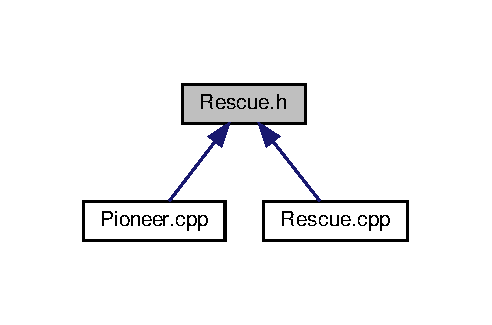
\includegraphics[width=236pt]{Rescue_8h__dep__incl}
\end{center}
\end{figure}
\subsection*{Estructuras de datos}
\begin{DoxyCompactItemize}
\item 
class \hyperlink{classRescue}{Rescue}
\begin{DoxyCompactList}\small\item\em Controlador de un robot de busqueda y localización de dos personas en distintos tipos de escenarios. \end{DoxyCompactList}\end{DoxyCompactItemize}
\subsection*{defines}
\begin{DoxyCompactItemize}
\item 
\#define \hyperlink{Rescue_8h_ac2cd96d53dd3ba6407db6766c3d92b26_ac2cd96d53dd3ba6407db6766c3d92b26}{M\+A\+X\+\_\+\+S\+P\+E\+ED}~100
\begin{DoxyCompactList}\small\item\em Máxima velocidad de las ruedas del robot. \end{DoxyCompactList}\item 
\#define \hyperlink{Rescue_8h_a3bfa6c68d124846bd629eef1504b2556_a3bfa6c68d124846bd629eef1504b2556}{N\+U\+M\+\_\+\+D\+I\+S\+T\+A\+N\+C\+E\+\_\+\+S\+E\+N\+S\+OR}~16
\begin{DoxyCompactList}\small\item\em Numero de sensores ultrasonidos que dispone el robot. \end{DoxyCompactList}\end{DoxyCompactItemize}


\subsection{Documentación de los \textquotesingle{}defines\textquotesingle{}}
\mbox{\Hypertarget{Rescue_8h_ac2cd96d53dd3ba6407db6766c3d92b26_ac2cd96d53dd3ba6407db6766c3d92b26}\label{Rescue_8h_ac2cd96d53dd3ba6407db6766c3d92b26_ac2cd96d53dd3ba6407db6766c3d92b26}} 
\index{Rescue.\+h@{Rescue.\+h}!M\+A\+X\+\_\+\+S\+P\+E\+ED@{M\+A\+X\+\_\+\+S\+P\+E\+ED}}
\index{M\+A\+X\+\_\+\+S\+P\+E\+ED@{M\+A\+X\+\_\+\+S\+P\+E\+ED}!Rescue.\+h@{Rescue.\+h}}
\subsubsection{\texorpdfstring{M\+A\+X\+\_\+\+S\+P\+E\+ED}{MAX\_SPEED}}
{\footnotesize\ttfamily \#define M\+A\+X\+\_\+\+S\+P\+E\+ED~100}



Máxima velocidad de las ruedas del robot. 



Definición en la línea 22 del archivo Rescue.\+h.

\mbox{\Hypertarget{Rescue_8h_a3bfa6c68d124846bd629eef1504b2556_a3bfa6c68d124846bd629eef1504b2556}\label{Rescue_8h_a3bfa6c68d124846bd629eef1504b2556_a3bfa6c68d124846bd629eef1504b2556}} 
\index{Rescue.\+h@{Rescue.\+h}!N\+U\+M\+\_\+\+D\+I\+S\+T\+A\+N\+C\+E\+\_\+\+S\+E\+N\+S\+OR@{N\+U\+M\+\_\+\+D\+I\+S\+T\+A\+N\+C\+E\+\_\+\+S\+E\+N\+S\+OR}}
\index{N\+U\+M\+\_\+\+D\+I\+S\+T\+A\+N\+C\+E\+\_\+\+S\+E\+N\+S\+OR@{N\+U\+M\+\_\+\+D\+I\+S\+T\+A\+N\+C\+E\+\_\+\+S\+E\+N\+S\+OR}!Rescue.\+h@{Rescue.\+h}}
\subsubsection{\texorpdfstring{N\+U\+M\+\_\+\+D\+I\+S\+T\+A\+N\+C\+E\+\_\+\+S\+E\+N\+S\+OR}{NUM\_DISTANCE\_SENSOR}}
{\footnotesize\ttfamily \#define N\+U\+M\+\_\+\+D\+I\+S\+T\+A\+N\+C\+E\+\_\+\+S\+E\+N\+S\+OR~16}



Numero de sensores ultrasonidos que dispone el robot. 



Definición en la línea 18 del archivo Rescue.\+h.


%--- End generated contents ---

% Index
\backmatter
\newpage
\phantomsection
\clearemptydoublepage
\addcontentsline{toc}{chapter}{Índice}
\printindex

\end{document}
